\chapter{Experiments and Evaluations\label{cha:chapter4}}

To evaluate Frankenbot's modular architecture based on the user experience, the surveys have been conducted. 
\\~\\
For evaluation of this research, a link provided in Appendix \ref{appen:deplFrank} to the deployed chatbot has been shared with participants using different social platforms along with an introductory text about the purpose of the study. Random users were selected irrespective of their profession, study background, and any race or gender discrimination. But the age limit constraint was set to be above 18. As participants were considered to be accused of a robbery and have to chat with a detective bot and answer his questions which can be a bit strict and straight forward for youngsters below 18. So the participant who participated with the minimum age was 22. On the contrary, the one with the maximum age was 34. And the average age calculated as 25.65 with a standard deviation of 2.37. Visuals have been shown in Figure \ref{fig:ageGraph}.

\begin{figure}[!h]
    \centering
    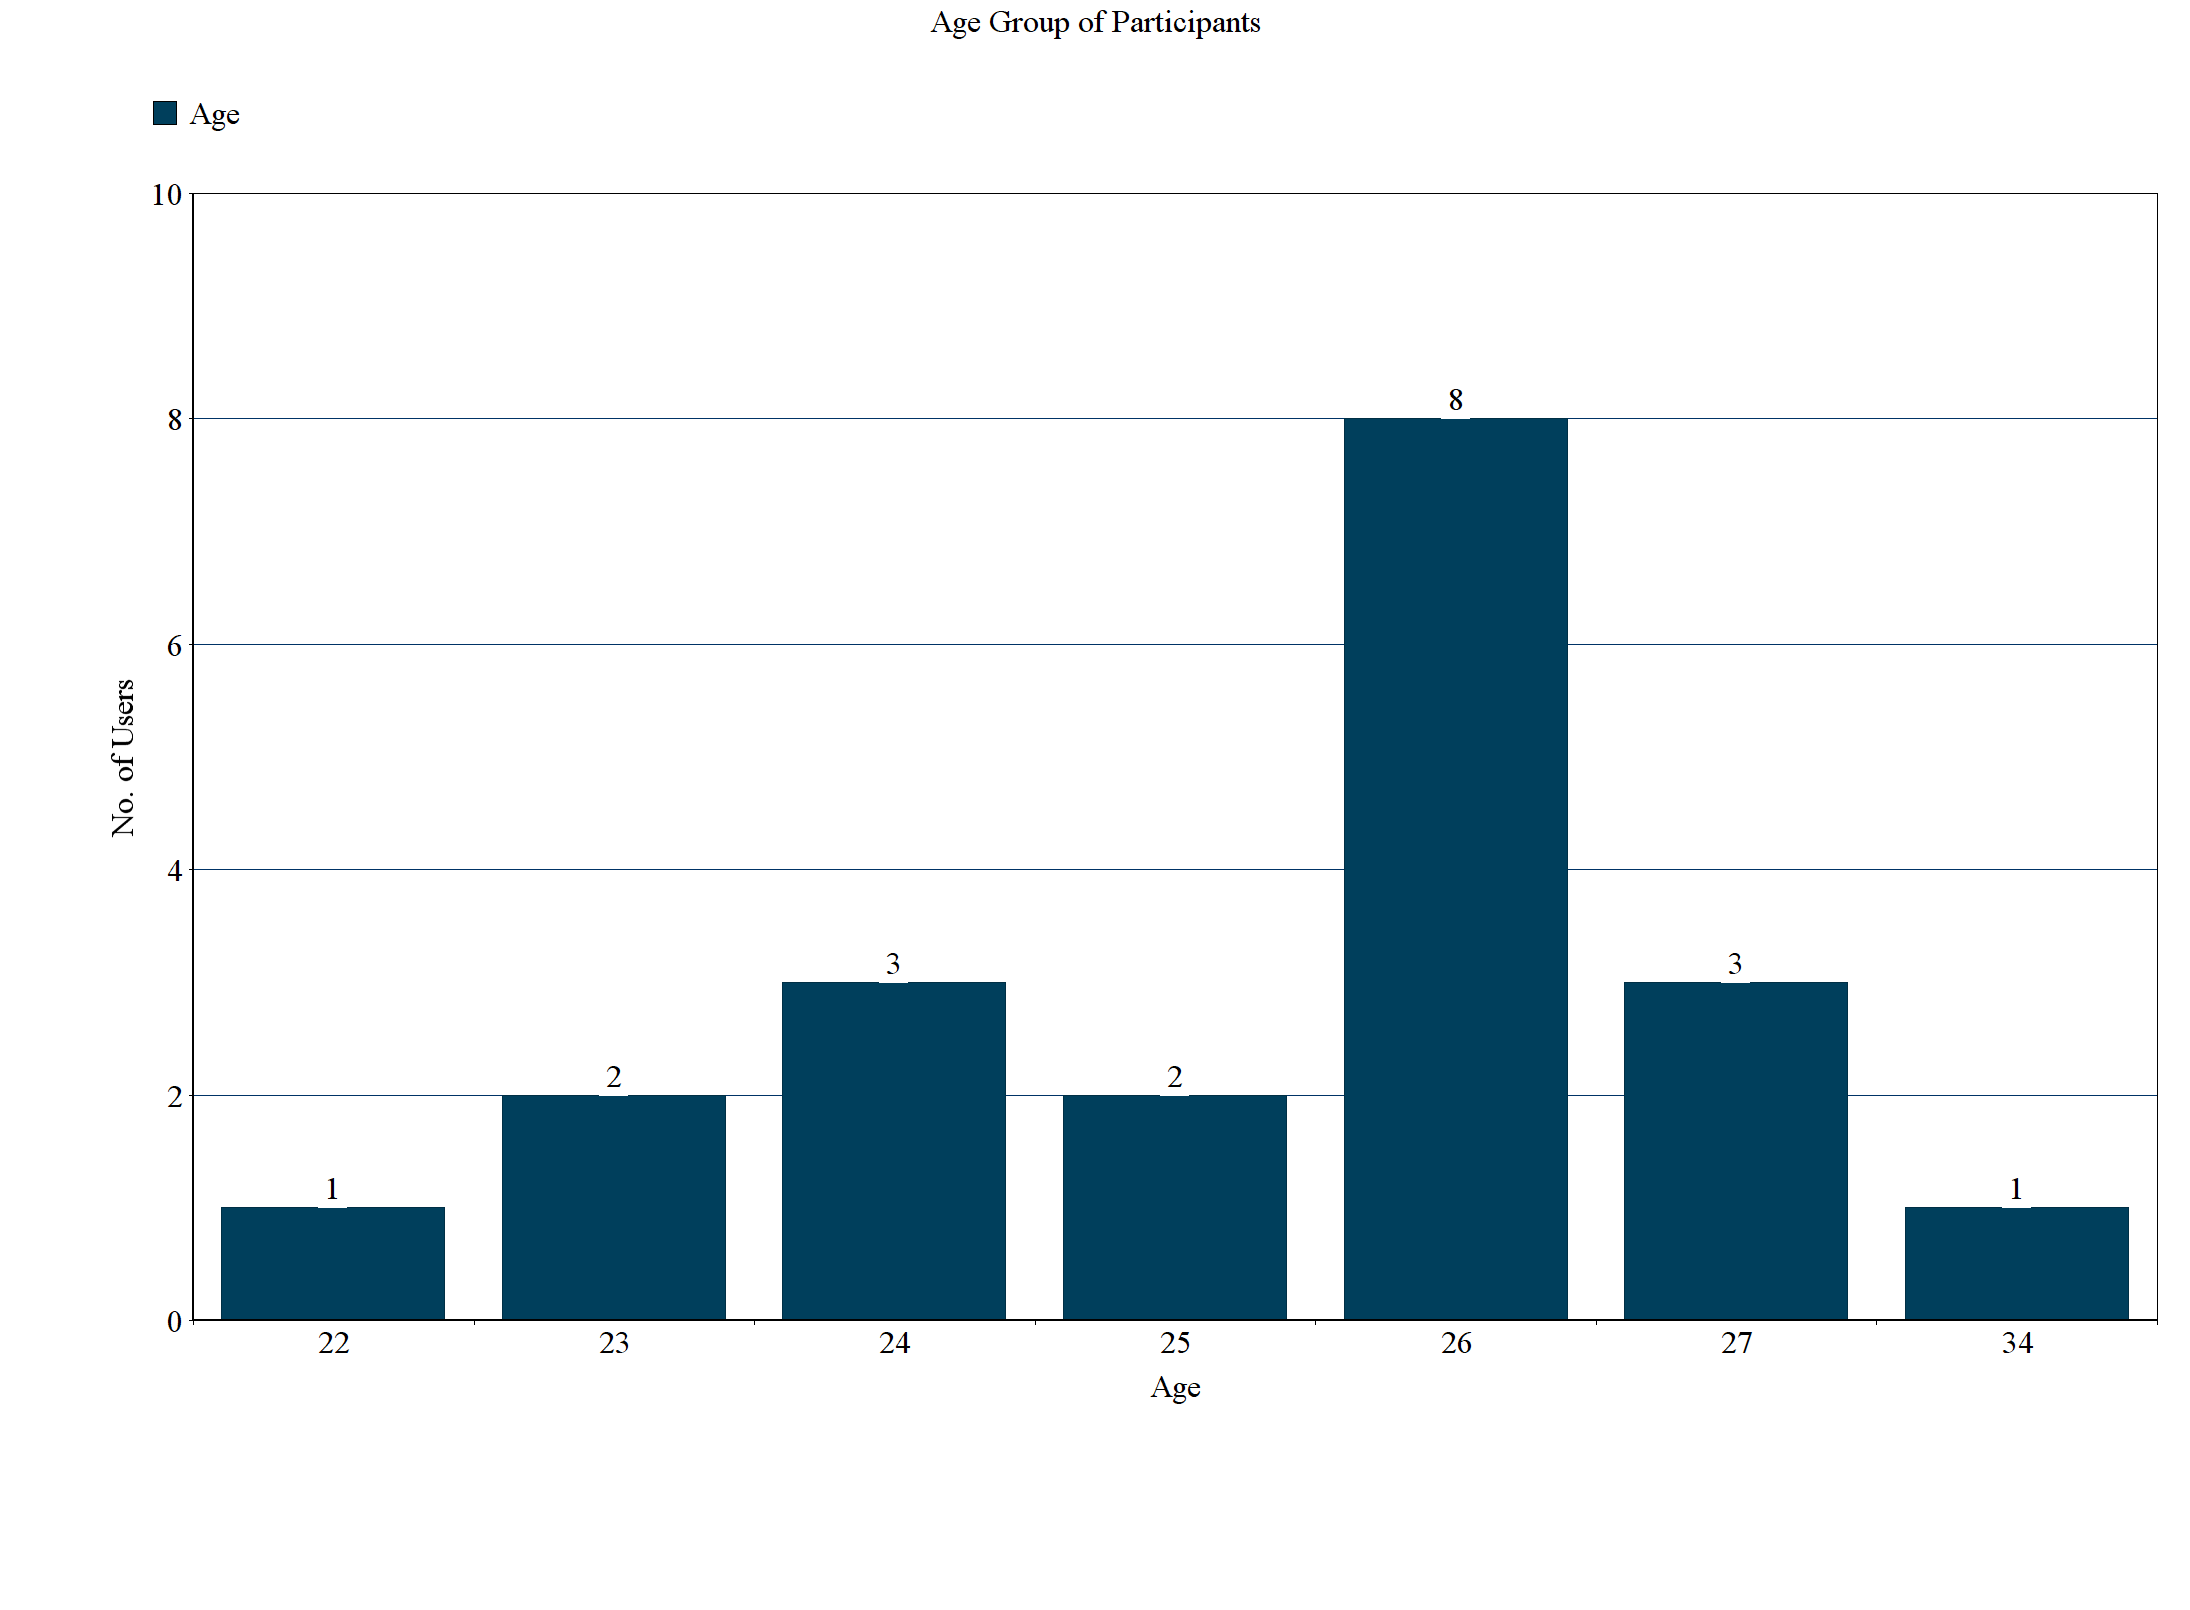
\includegraphics[width=0.9\textwidth]{img/Age_Graph_Updated.PNG}
    \caption{Age stats of participants}
    \label{fig:ageGraph}
\end{figure}
\\~\\
Figure \ref{fig:profGraph} depicts that a total of 20 users participated in this study. Most of them appeared to be from a technical background as a maximum of them appeared to be students from different universities. The second majority of participants revealed themselves as IT employees. While remaining revealed themselves as teacher and business qualified.

\begin{figure}[!h]
    \centering
    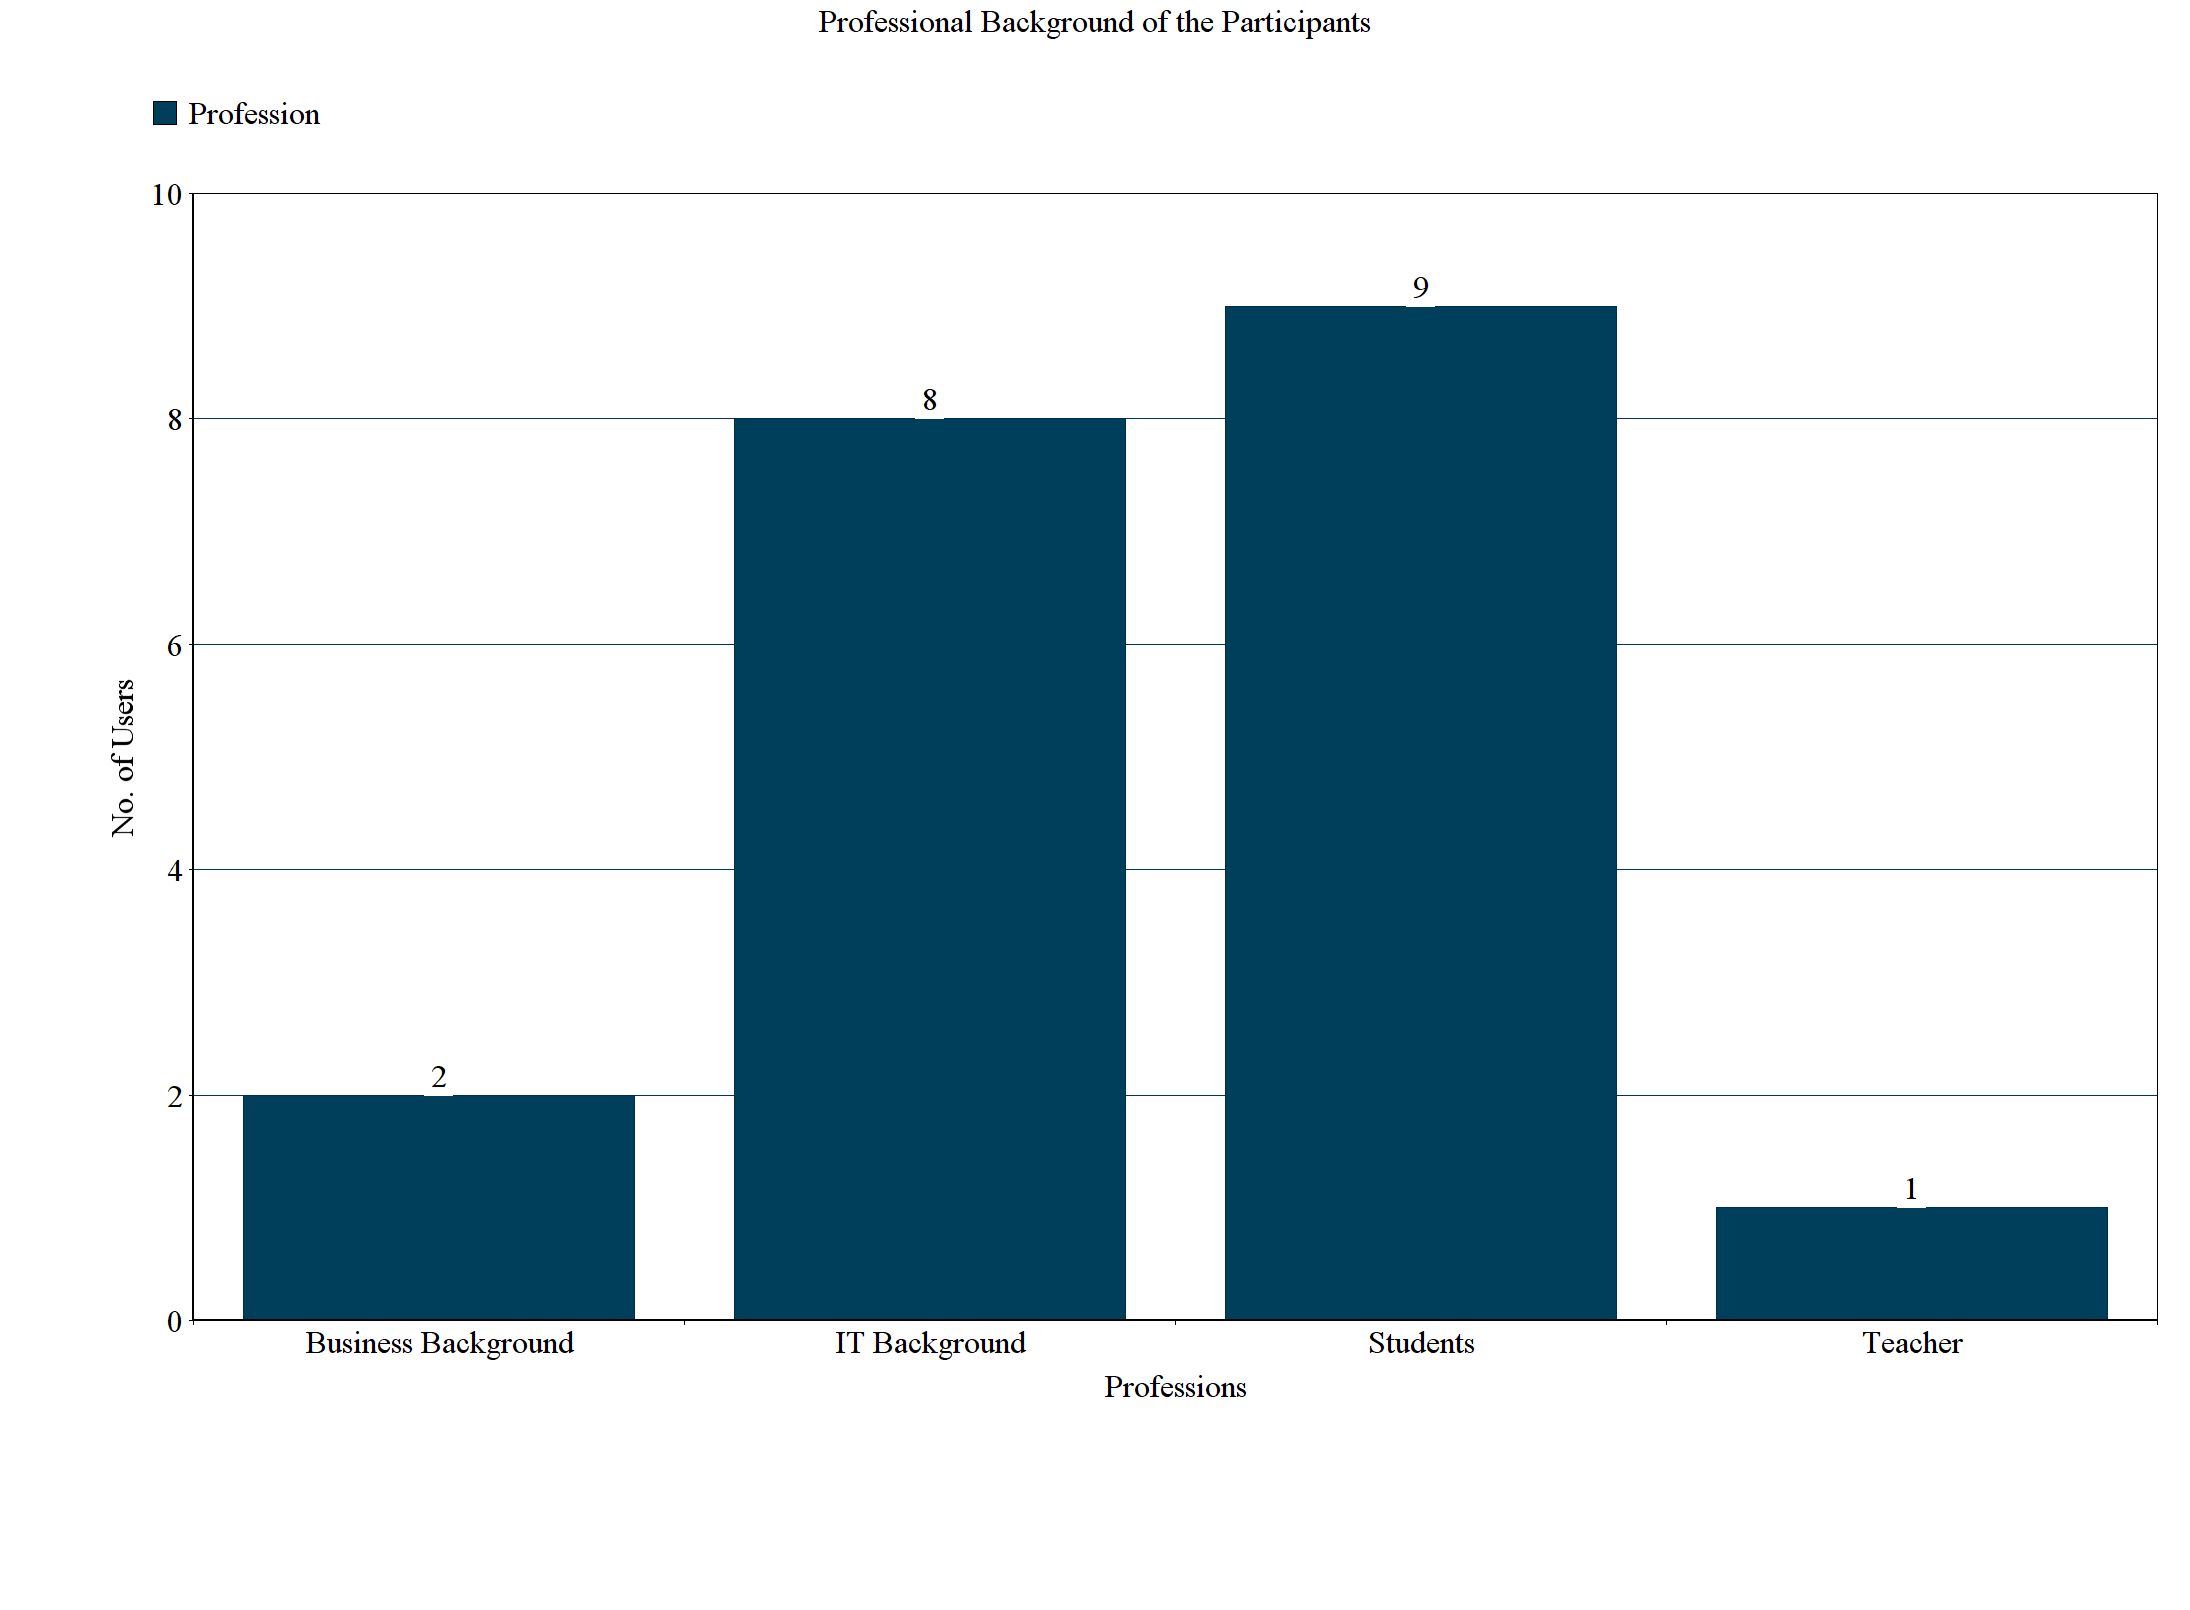
\includegraphics[width=0.9\textwidth]{img/Profession_Graph_Updated.PNG}
    \caption{Profession related details of participants}
    \label{fig:profGraph}
\end{figure}

\section{Conducted Surveys}
All participants were asked to complete two surveys. One named as "Frankenbot's Experience Survey" was designed with the help of \cite{evaluatingSpokDialSys}\cite{itut}. For the second survey, the standardized tool to personally evaluate the usability and design of an interactive product known as AttrakDiff \cite{attrakdiff} has been used. The first survey was designed using Google Forms and the purpose of it was to capture the user's interaction experience about the Frankenbot. While the purpose of AttrakDiff's study was to evaluate different aspects such as Frankenbot's utility and usability. Furthermore, it also helped to weigh the chatbot for task-oriented and self-oriented qualities. 
\\~\\
The users were provided with the link to the deployed chatbot's interface as a web page and they can easily access it from their places. It provided ease to the user and enhanced the comfortability factor for them. Also, they have to read the description and instructions provided for them on the web page. And they have to figure out what to do and how to operate the chatbot on their own without any external help. Which has given more realistic and unbiased essence to the results obtained.
\\~\\
For the surveys, the web page contains the heading "Frankenbot's Request" in which the users were requested to complete the surveys. Once, they are finished having chat for a fun purpose with the chatbot then they could visit the hyperlinks provided for both of the surveys.
\\~\\
The surveys were conducted in the English language. Whereas, AttrakDiff's survey has the option for both English and German. You can find "Frankenbot's Experience Survey" in Appendix \ref{appen:survey}. Furthermore, AttrakDiff's Single Evaluation Study\cite{indeval} has been used as the second survey.
\\~\\
The questionnaires were filled by the participants on their own devices. While a user was interacting with the chatbot all communication was getting stored into the log file for future records and usage.

\section{Experimental Setup}
This research study has been conducted to gather the results for what the user has experienced while interacting with the chatbot. The whole experiment itself has been divided into four major parts mentioned below:
\begin{enumerate}
    \item Explanation of the chatbot for the participants to make it's testing successful.
    \item Participants were requested for accomplishing a set of tasks with the chatbot.
    \item The questionnaire to collect the user's interaction experience about the chatbot named as "Frankenbot's Experience Survey".
    \item Quality evaluation of the chatbot via AttrakDiff's Single Evaluation.
    \item Short interview of the participants.
\end{enumerate} 
All of these are explained underneath in detail.

\subsection{Explanation of the Chatbot}
Users were provided with the description and instructions on the web page about the chatbot. The following sub-sections contain the required information and directions for the users to operate the chatbot. Visual representation has been displayed in Figure \ref{fig: userInter}.

\subsubsection*{Information}
Real information provided to the participants has been provided in Appendix \ref{appen:info}. They were provided with the introduction about the Frankenbot that it is the detective chatbot designed to interrogate you about the armed robbery that happened a few days back at a spatkauf near Berliner Strasse. It is responsible for investigating, so it is going to ask you some questions to come up with a decision. It will include, what it has investigated so far. Also, you can have a general conversation with it like you can ask it to talk about general stuff with you, about corona virus and its stats, to make you laugh, to do gossips, how does it feel, who is it, what does it eat and other related questions about the chatbot. You can switch between the topics at any moment as it is designed for parallel handling of multiple topics. Kindly, communicate with it until it reaches any decision or says you goodbye before you jump to completion of the surveys.
\\~\\
Lastly, the ending of the information provided a brief note about how to re-initiate the chat. If a user gets lost in between the dialogue and wants to reinstate the detective game then just send a greeting message (hi, hello, etc.) and the chatbot will restart it for him/her. 

\subsubsection*{Instructions}
Actual instructions are stated in Appendix \ref{appen:instr}. The user was asked to think as he/she is accused of a robbery and sitting in front of a detective and have to answer his deceptive questions to prove his/her innocence. Otherwise, he/she will be declared as a culprit. It is the responsibility of a detective to make a decision based on the user's answers to his questions.
\\~\\
At the end of the instructions, there was a small notice available for the user to remove his/her doubts about its reality that it is the fictional detective chatbot designed only for testing and fun purpose.

\subsection{Tasks}
The participants were requested to accomplish the following tasks beforehand, to fill the surveys.
\begin{itemize}
    \item Users were requested to play a small game with the detective chatbot and answer the questions, the way they wanted.
    \item They were also informed that they could have a general dialogue with the chatbot. They could also talk to it about general stuff, corona virus and its stats, to tell a joke, to do gossips, query about its feelings and emotions and other related questions.
    \item Additionally, they were also notified that they can switch the topics. This means they can start talking about general stuff if they are talking to the detective bot and vice versa by just replying to the last question of the previous topic.
    \item Lastly, they were requested not to leave the conversation in between until they reach the ending of the detective game. 
\end{itemize} 
\\~\\
All users were requested to chat with the chatbot at minimum until it came up with any decision or says goodbye. Other than that, there was no time restriction for them and they could have a dialogue for as long as they desired to.

\subsubsection*{Frankenbot's Request}
Finally, the user was requested as stated in Appendix \ref{appen:req} that once he/she has finished interaction with the chatbot, please don't forget to complete two of the assessments demonstrated in the Appendix \ref{appen:survey}. They were allowed to start with it after 1 minute of web page activation at a minimum. Meanwhile, a user should get familiar with the chatbot by chatting with it. Frankenbot also stated that it welcomes and highly appreciates the user's prestigious feedback which will help its developer to get it evaluated and enhance its abilities for a better experience.

\subsection{Interview\label{subsec:interview}}
In the end, a brief interview was conducted after having their consent. And not all the users permitted it but 12(60\%) of the participants showed their availability for a small session. The users have been verbally asked the following questions:
\begin{itemize}
    \item Whether they faced any problem to make chatbot understand their messages?
    \item Did they reach the end of detective game i.e. a chatbot declared them culprit or responded them with bye message?
    \item Whether chatbot guided them well in case of any confusion that how to proceed ahead?
    \item Did they enjoy the communication?
    \item Did they try with switching the topics?
    \item Whether they liked the detective game or not?
    \item Whether they liked the user interface or not?
\end{itemize}

\subsection{Frankenbot's Experience Questionnaire}
When the user completed the tasks allocated to him/her then he/she filled out the questionnaire about his/her interaction with the chatbot. The questionnaire is shown in Appendix \ref{appen:expsurvey} has been divided into the following sections:
\begin{itemize}
    \item Users' overall impression about the interaction with the chatbot.
    \item Familiarity of the user with the already existing chatbots.
    \item Whether the user succeeded to achieve the desired goals.
    \item How was the communication with the chatbot.
    \item What was the behavior of the chatbot with the users.
    \item How well the dialogue was designed.
    \item Personal impression and user's experience about the chatbot.
    \item Users' opinions about the chatbot's usability. 
\end{itemize} 
All sections have consisted of several questions. And the user has to respond by selecting an option out of the linear scale from 1 to 5 whether he/she strongly agrees, agrees, undecided, disagrees or strongly disagrees with it. Most of the questions needed to be answered using these five options. Other than that overall impression about the chatbot has been measured using the linear scale of 5 options starting from 1 and ending on 5 as excellent, good, fair, poor, and bad.

\subsection{AttrakDiff Single Evaluation}
After completing the Frankenbot's Experience Survey, users have been requested to complete the AttrakDiff's standardized questionnaire to measure how the users perceived the design, quality, and usability of the chatbot.
\\~\\
The AttrakDiff is an institutional questionnaire that has been used to rate the products using the series of several word pairs \cite{alex}. Each word pair consists of the options as a linear scale from 1 to 7. Option at position 1 is a word while on number 7 there also exists a word but its acronym \cite{attrakdiffQuest}. These pairs of words are classified into three following categories: (i) Pragmatic Quality, it includes the word pairs like “cumbersome - straight forward” and “impractical - practical”. (ii) Hedonic Quality, the words pairs like “tacky - stylish” and “unimaginative - creative” lie under this category. And (iii) Attractiveness, word pairs such as “pleasant - unpleasant” and "ugly - attractive" are grouped under this attribute \cite{alex}.

\section{Quantitative Analysis}
This section contains the explanation and quantitative analysis of the results obtained during the research. It has been further divided into two steps: (i) The results for all the sections for the Frankenbot's Experience Survey as mentioned above and also the results for the AttrakDiff Single Evaluation stated before. 

\subsection{Frankenbot's Experience Survey}
It analyzes the results gathered about all the sections of the questionnaire.

\subsubsection*{Overall Impression}
This section includes a question about the user's overall impression about the interaction with the chatbot as pictured in Figure \ref{fig:overallImpre}. It has been measured using the linear scale of 5 options starting from 1 and ending on 5 as excellent, good, fair, poor, and bad. And out of the total 20 responses collected by the conduction of the survey, 2(10\%) responded with excellent mark and 9(45\%) rated it as good. So, a total of 11 out of 20 which is 55\% of the total participants, have passed positive remarks about it. Whereas, other 4(20\%) judged it as fair which also lies under the category of acceptable. So after summing up the percentages, 75\% of the participants rated their interaction as charming. On the contrary, out of the remaining participants, 3(15\%) rated it as poor and only 2(10\%) assigned it a bad label. So, it depicts that overall users' impressions about the interaction with the chatbot went well.

\begin{figure}[!h]
    \centering
    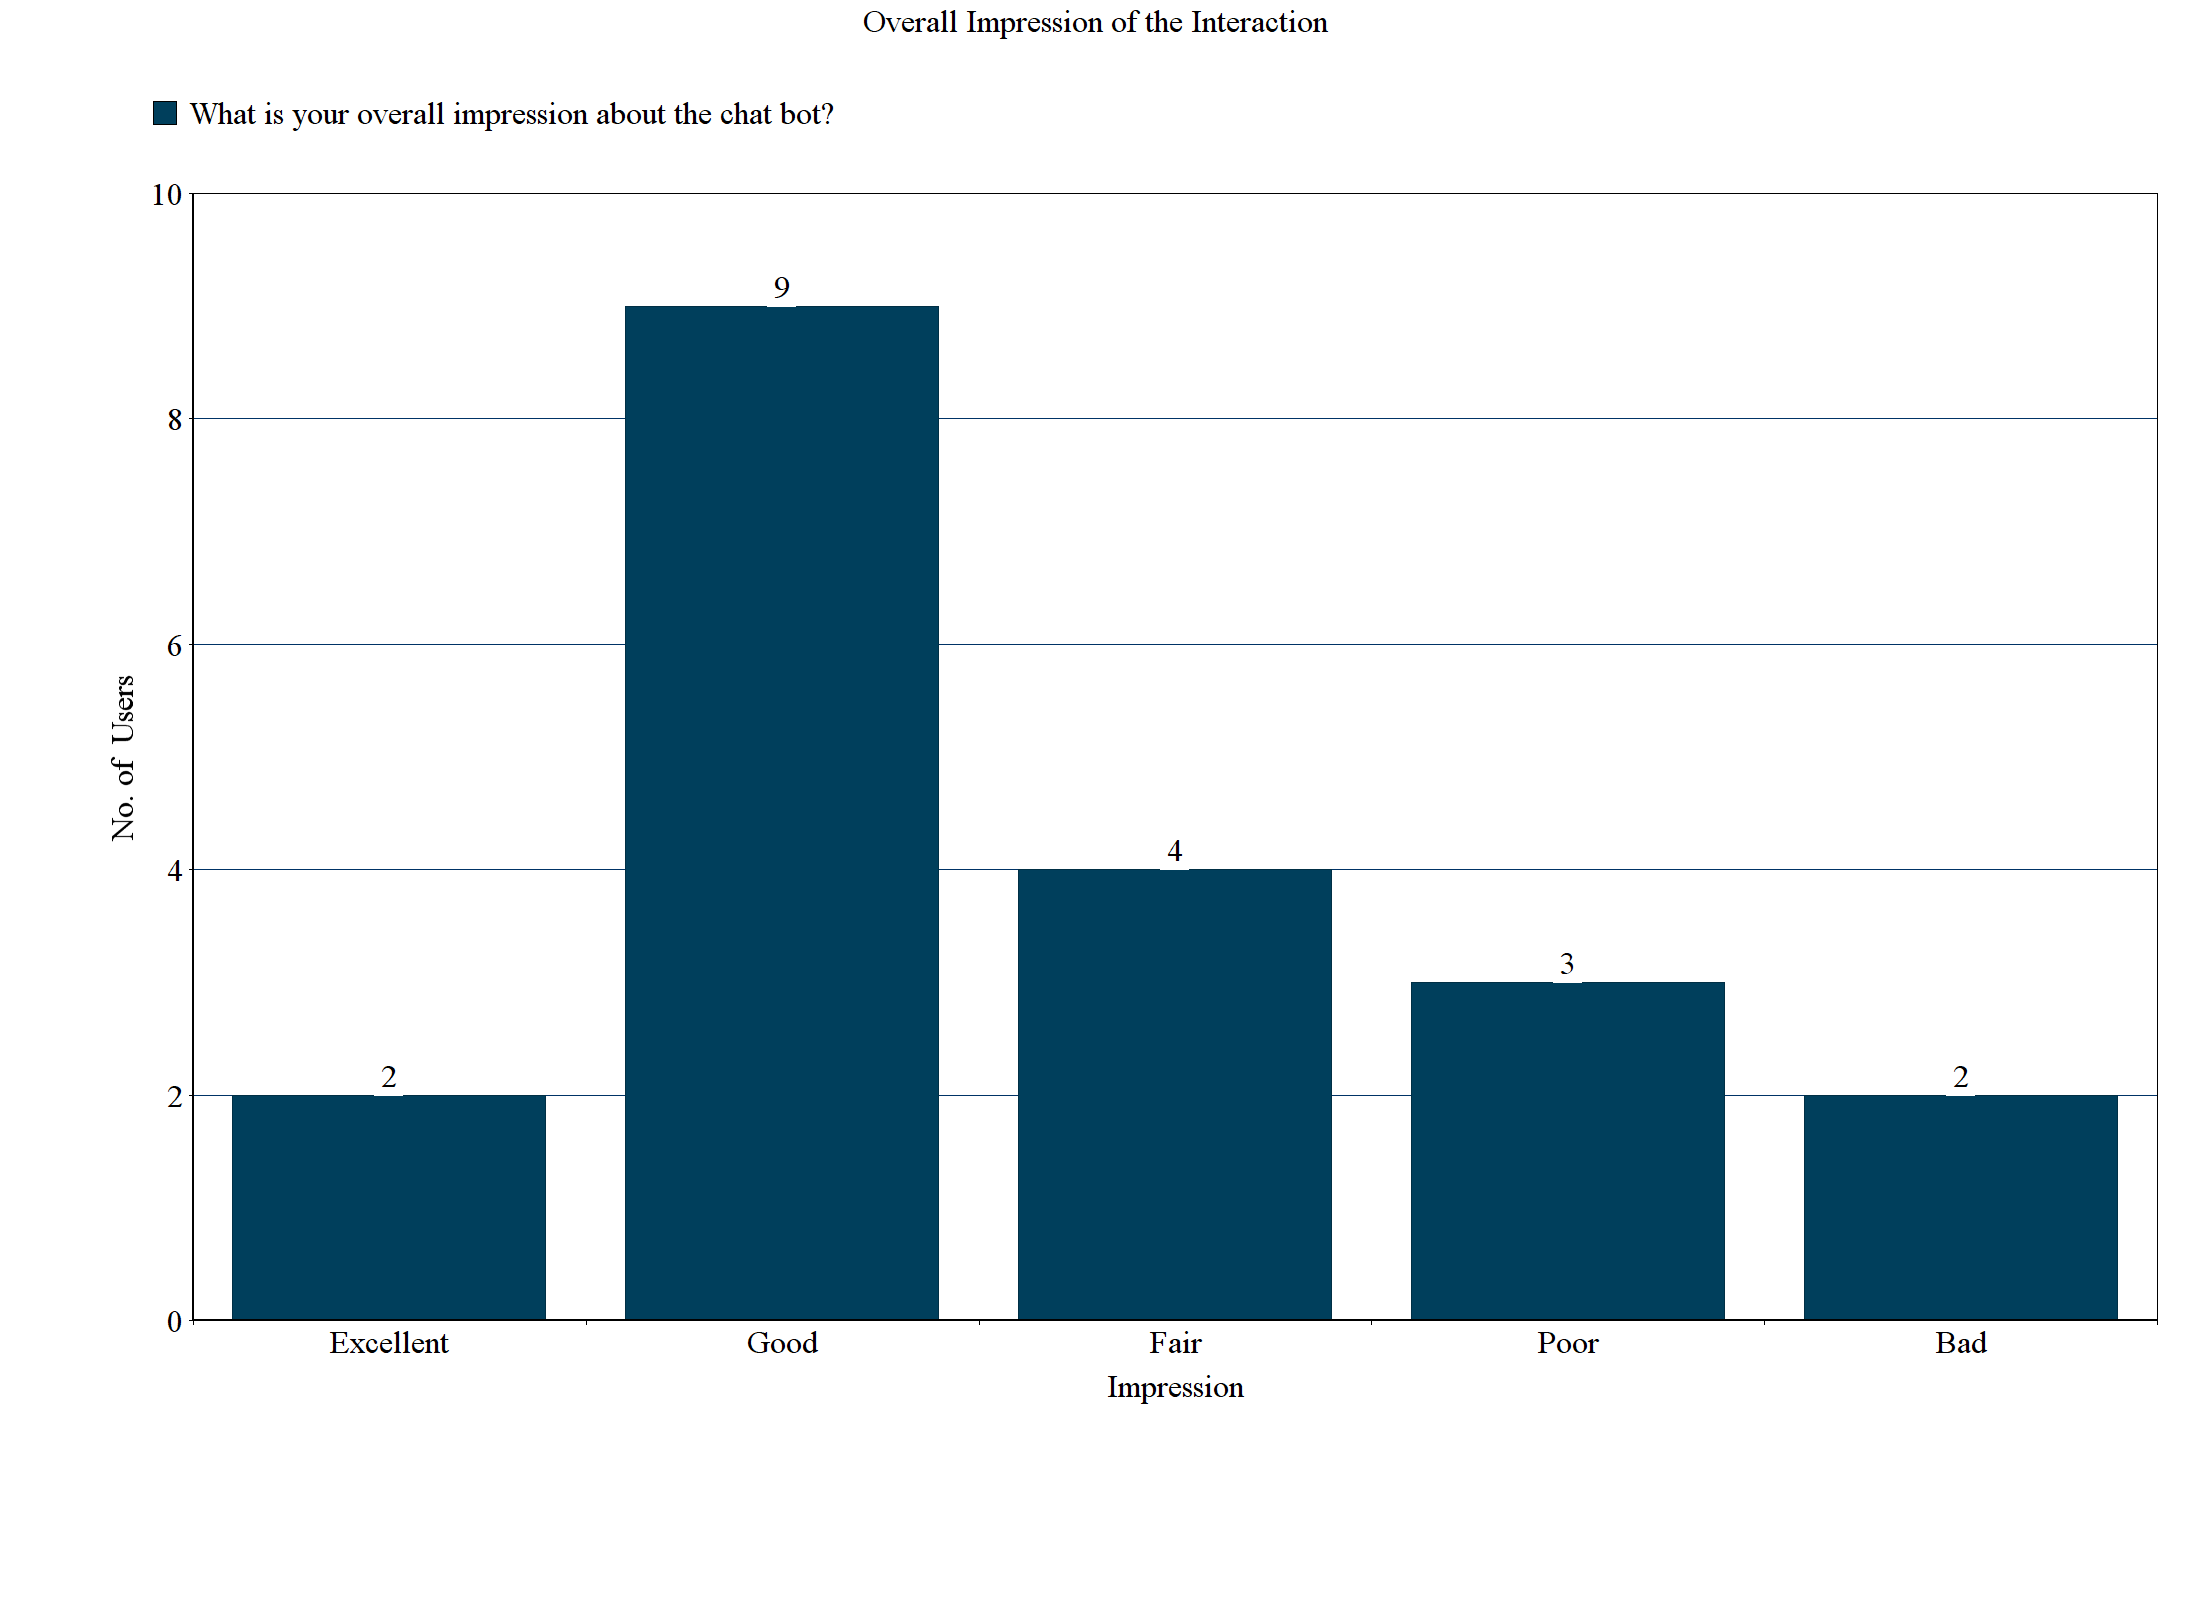
\includegraphics[width=0.9\textwidth]{img/Overall_Impression_Updated.PNG}
    \caption{Overall impression of the interaction with the chatbot}
    \label{fig:overallImpre}
\end{figure}

\subsubsection*{Familiarity with Existing Chat Bots}
This section added to the questionnaire just to figure out the experience of the participants with already existing chatbots. Whether they were well familiar with the chatbots or are inexperienced with this emerging technology. So that if the majority of them have a good knowledge of any of the existing chatbots, it will provide more strength and solidity to the results gathered from such participants.
\\~\\
There were a total of 3 questions available under this section of the survey attached in Appendix \ref{appen:expsurvey} that participants have to answer:
\begin{enumerate}
    \item I feel that I am well familiar with the chatbots like Google Assistant, Apple's Siri, etc. (Possible options lie between the scale of strongly agree to strongly disagree).
    \item I communicate with the chatbots. And the possible options provided were Frequently (daily or several times in a week), Seldomly (rarely in weeks or months), Just a few times and Never.
    \item Purpose of my chatbots usage is: (only if you answered a question no. 2 positively). Possible answers could be any out of the following: Personal commands to provide you assistance in performing tasks, For fun, Not feel lonely and No reason.
\end{enumerate}
Fortunately, for the first statement, 16(80\%) appeared to be well familiar with the existing chatbots. 2(10\%) answered with undecided and the remaining 2(10\%) just disagreed with the statement but no one strongly disagreed with it. Graph depicting such results has been shown in Figure \ref{fig:familiarity}. Coming to the second statement, 5(25\%) detected to be frequent users. 8(40\%) resulted to be the seldom users. Whereas, 6(30\%) communicated just a few times with the chatbots as shown in Figure \ref{fig:commChatRes}. Lastly, almost 60\% knew how to operate and give commands to the chatbot. And around 30\% appeared to use it for joy and fun purposes. These stats and readings portray that experienced users participated in this study. And the results obtained from the study are trustworthy and reliable. 

\begin{figure}[!h]
    \centering
    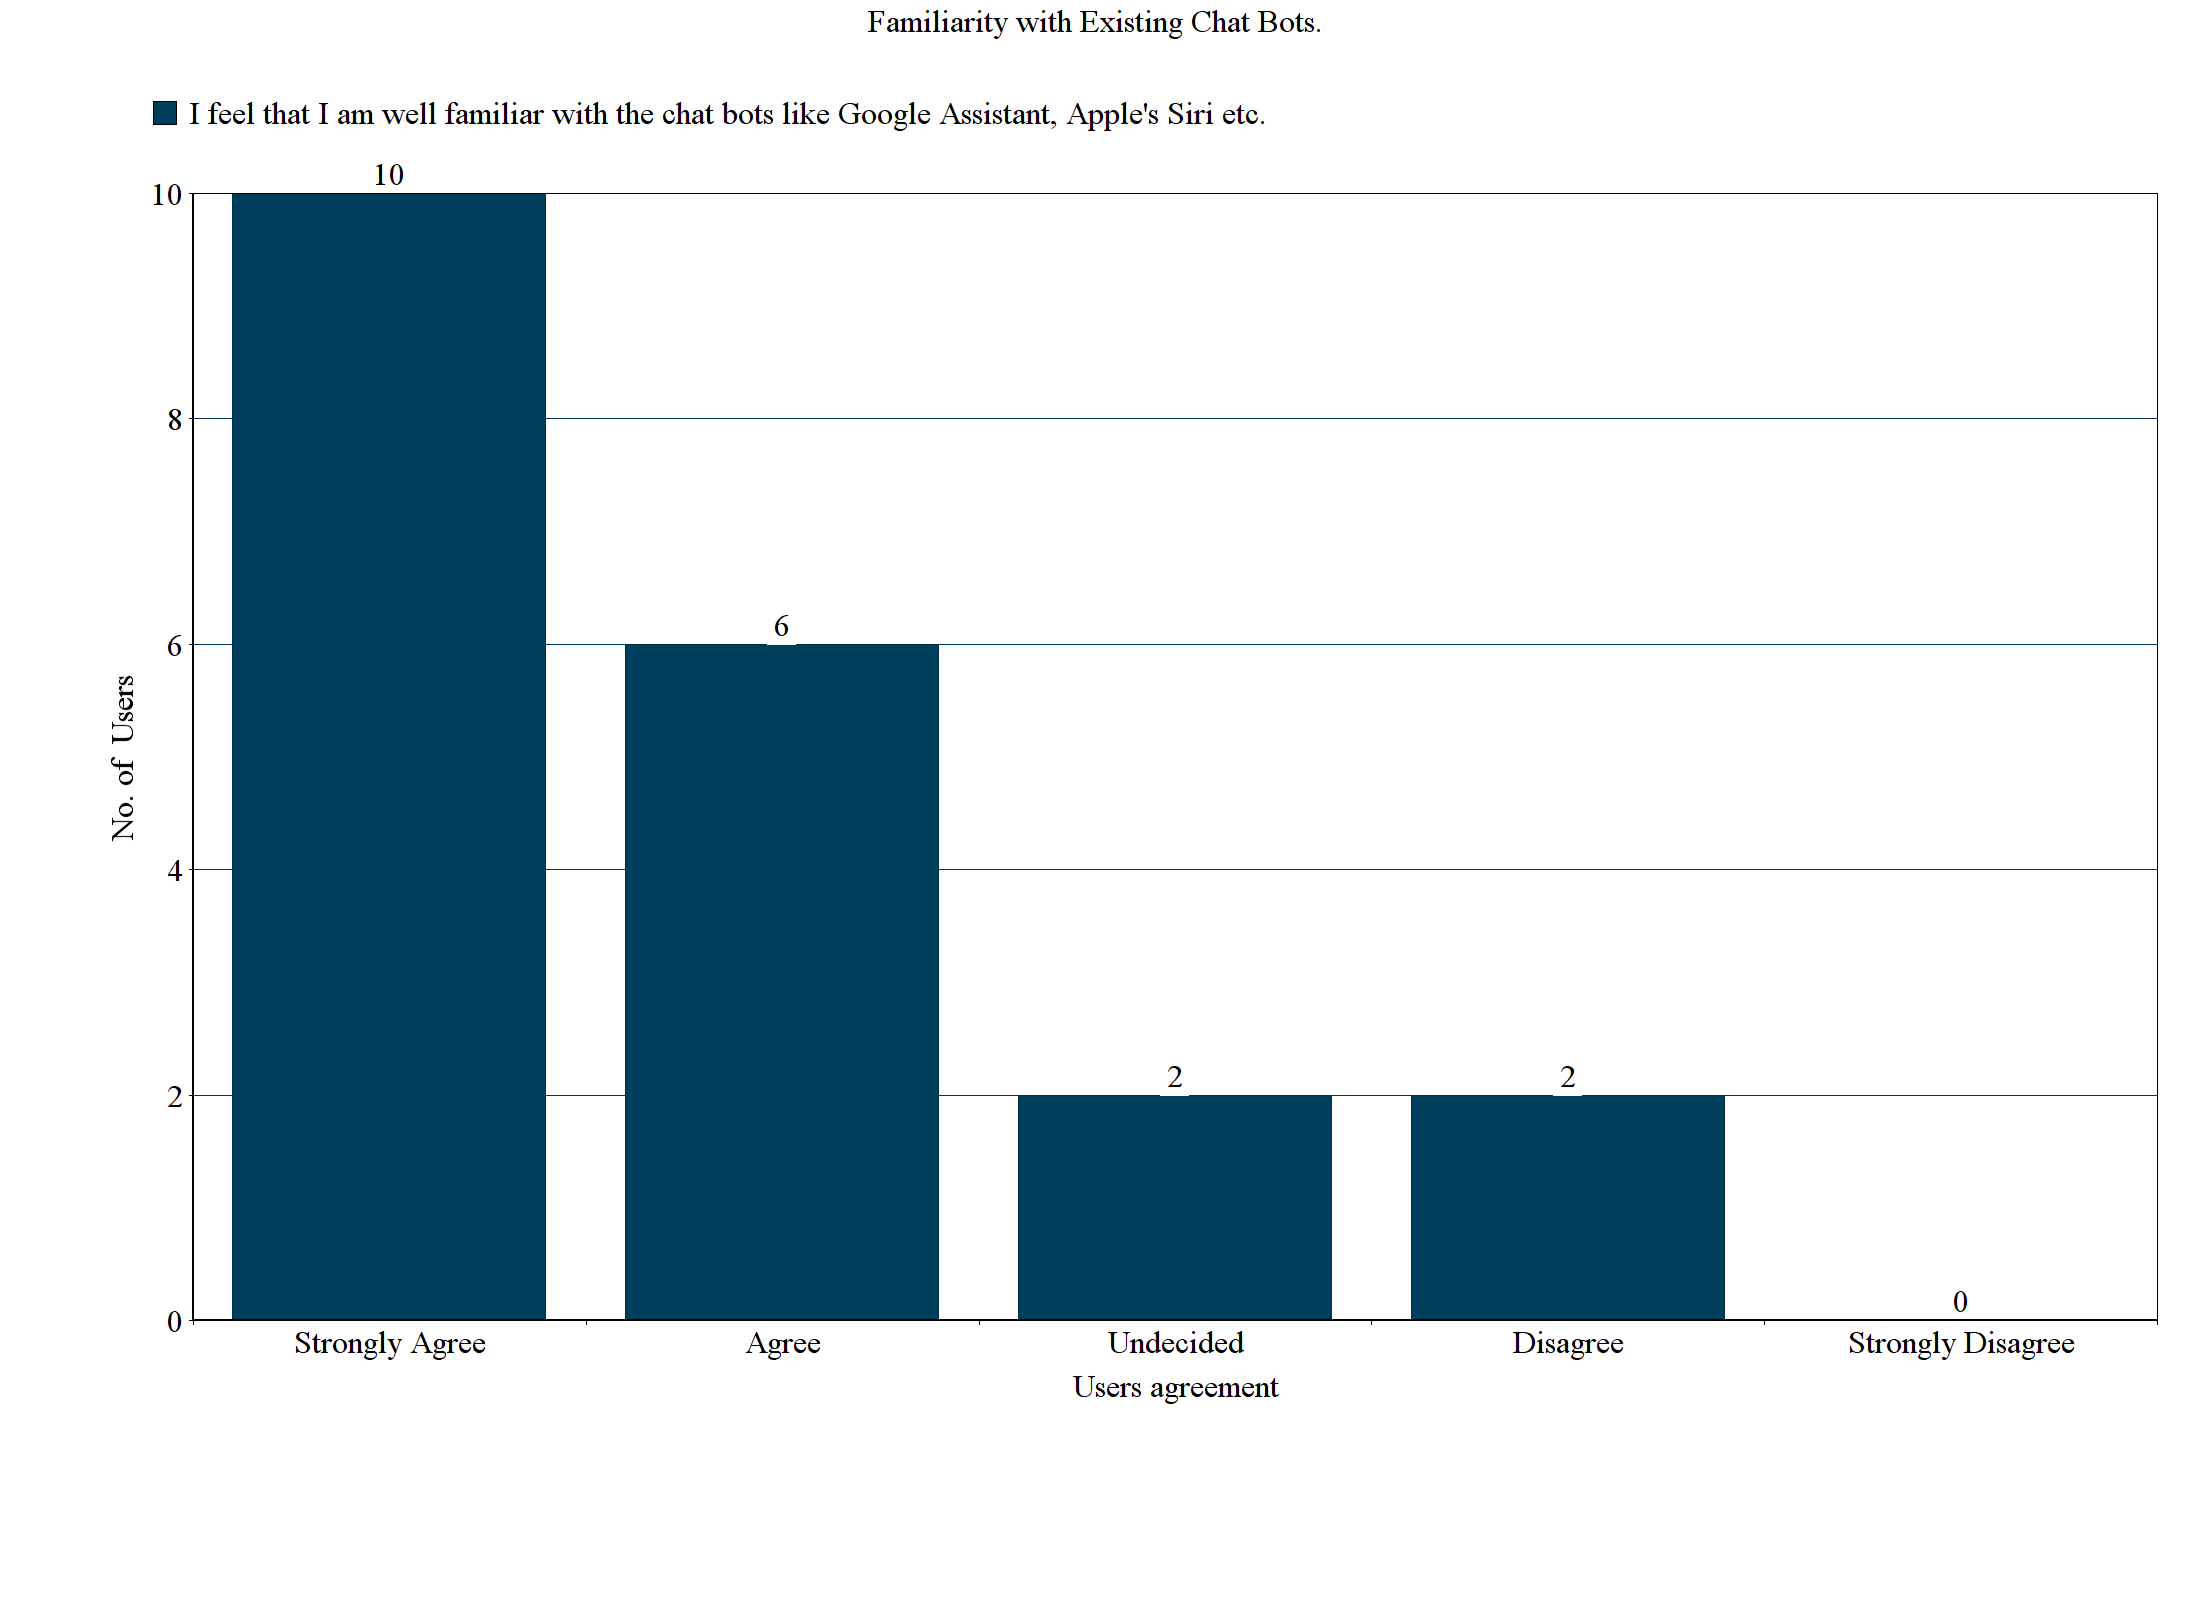
\includegraphics[width=0.9\textwidth]{img/Familiraity_Updated.PNG}
    \caption{Participants familiarity with the chat bots like Google Assistant, Apple's Siri etc.}
    \label{fig:familiarity}
\end{figure}

\begin{figure}[!h]
    \centering
    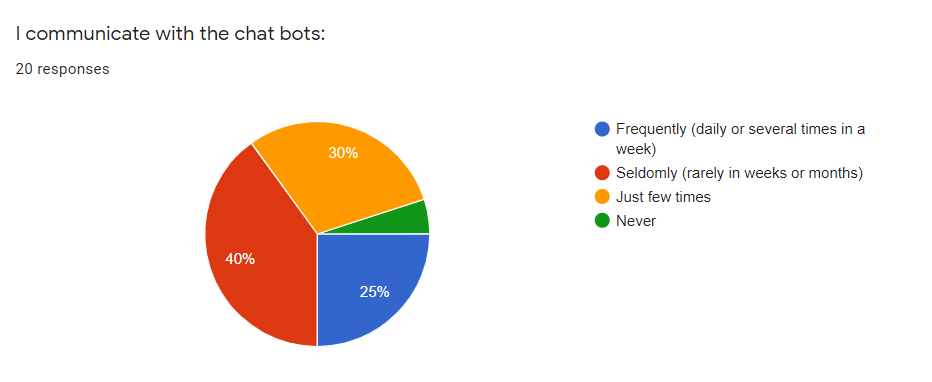
\includegraphics[width=0.9\textwidth]{img/Communicate_Chatbots_Result.PNG}
    \caption{Participants usage of the chat bots like Google Assistant, Apple's Siri etc.}
    \label{fig:commChatRes}
\end{figure}

\subsubsection*{Achievement of Goals}
It highlights whether the user succeeded to achieve the desired goals or not while having an interaction with the chatbot. It contained the following questions in responding to which user checked an option that varied from strongly agree to strongly disagree. Detailed comparison for all the answers collected for the following statements can be found in Figure \ref{fig:achievGoals}.
\begin{enumerate}
    \item The information provided by the chatbot was clear.
    \item The provided information was incomplete.
    \item The interaction with the chatbot was efficient.
    \item The chatbot is unreliable.
\end{enumerate}

\begin{figure}[!h]
    \centering
    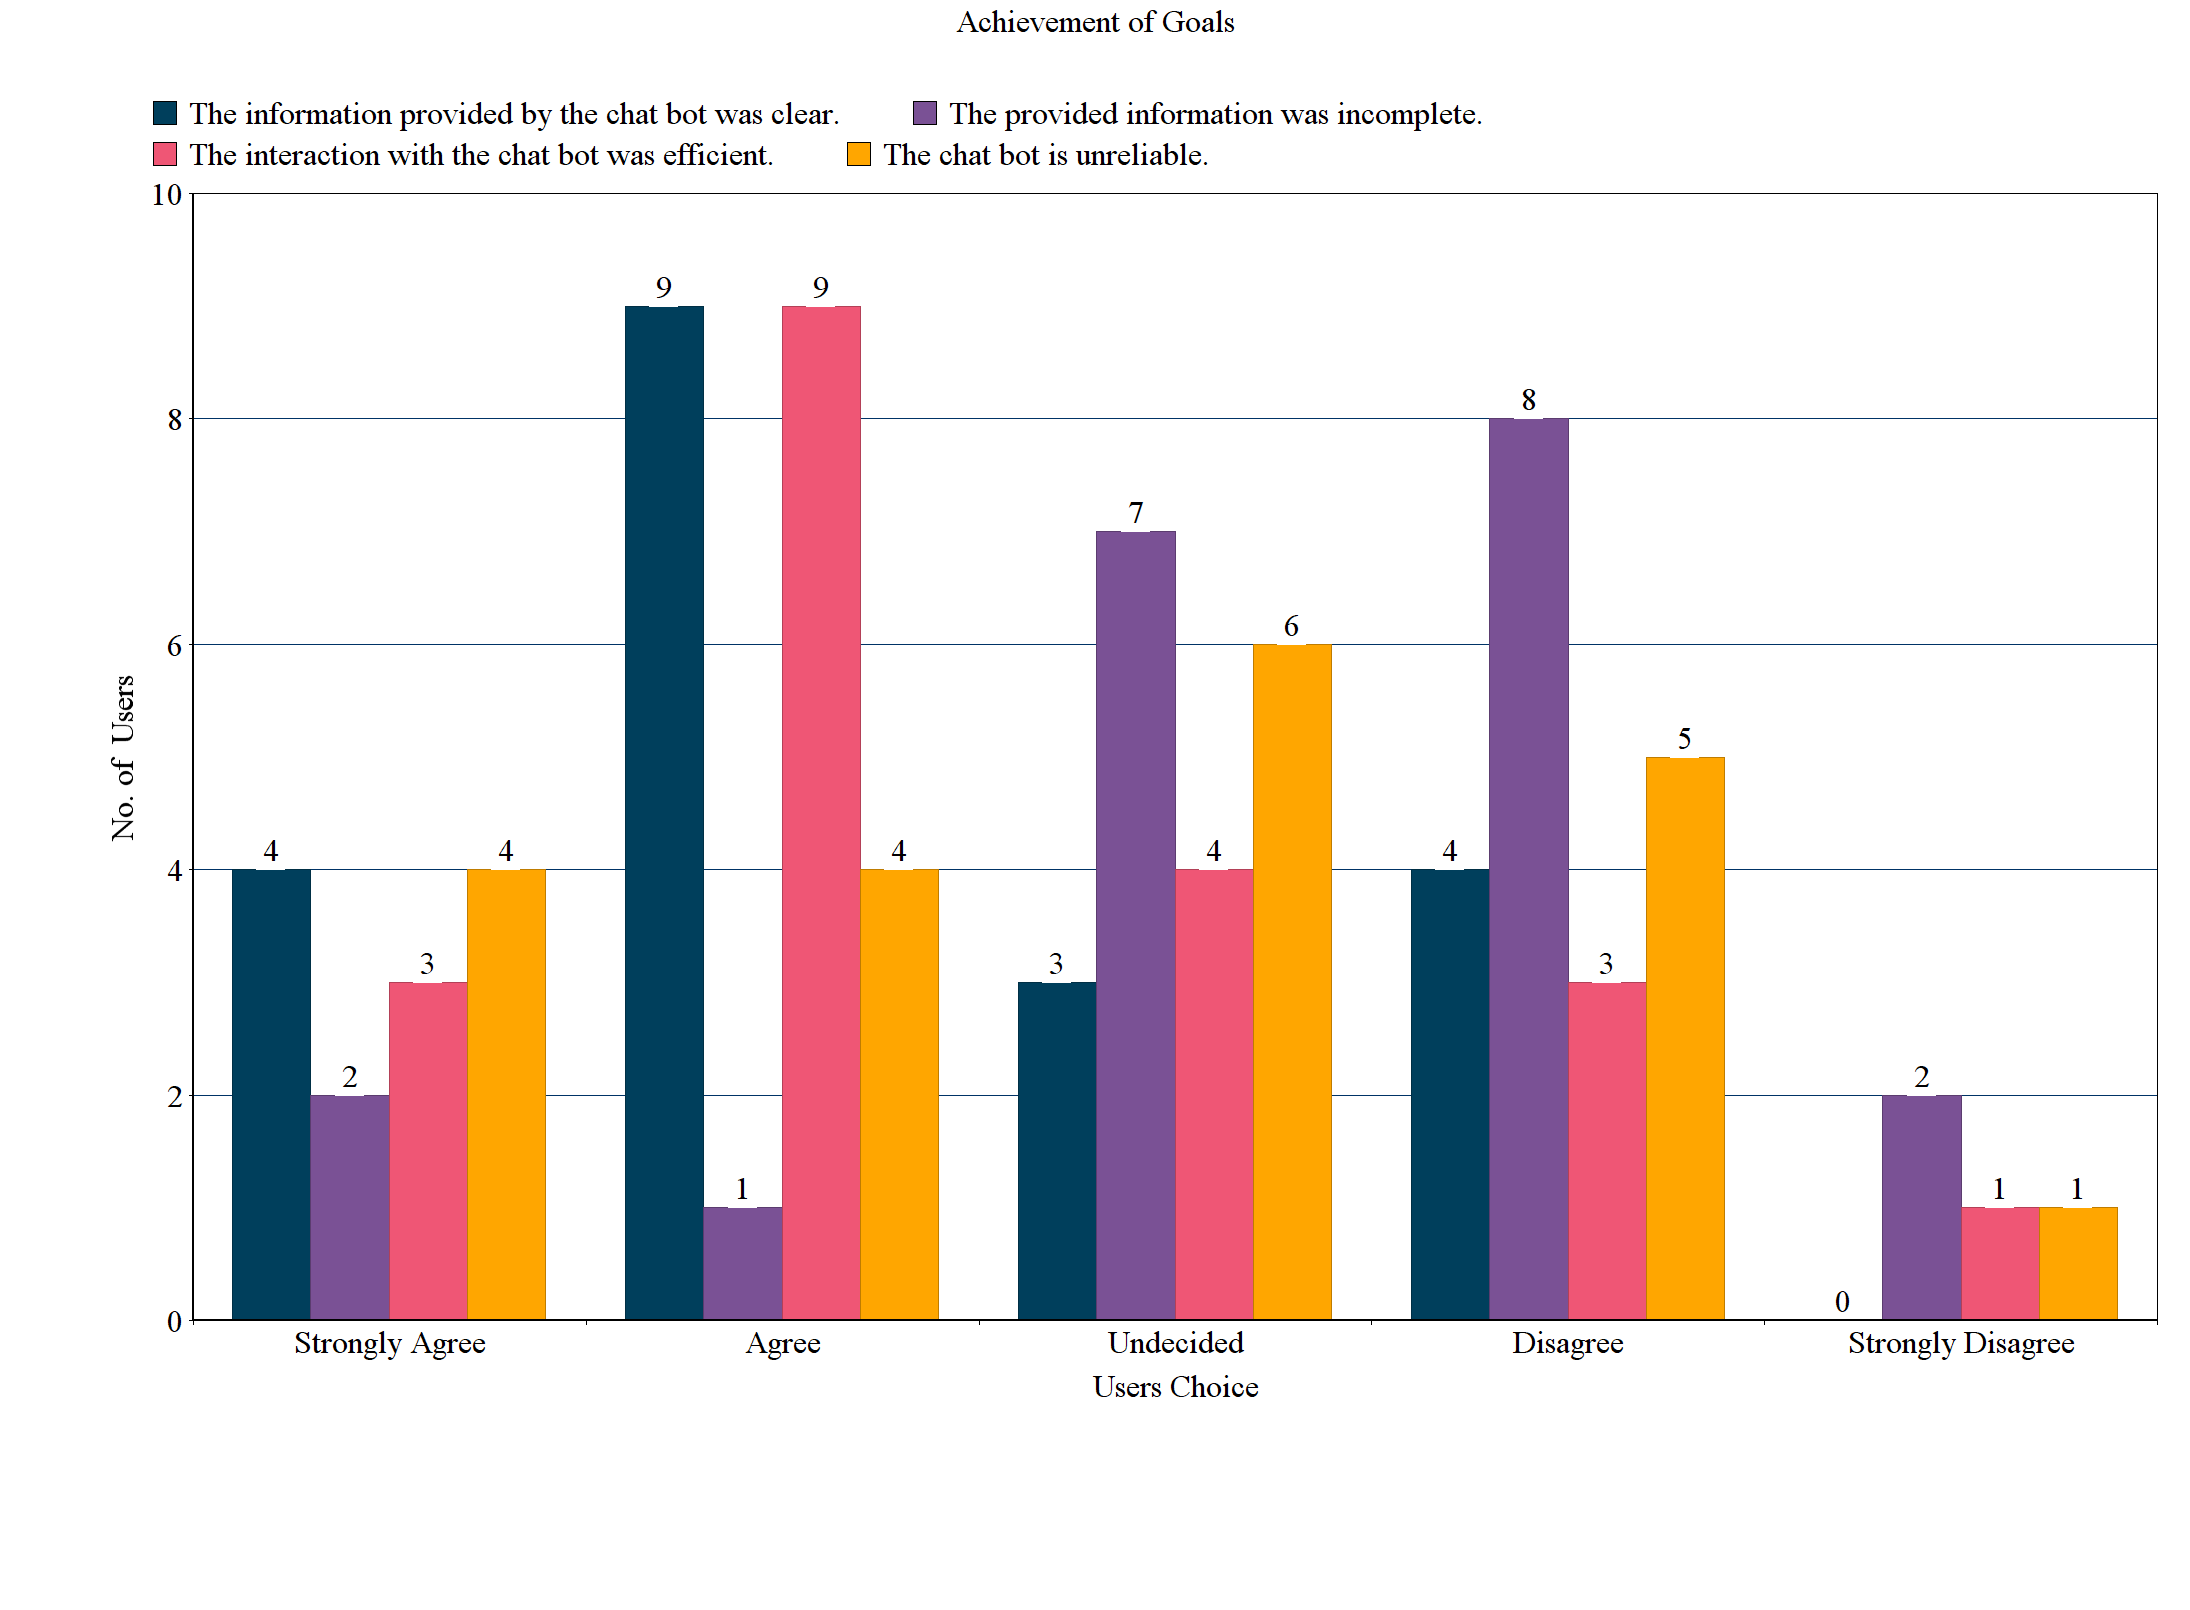
\includegraphics[width=0.9\textwidth]{img/Achievement_of_Goals_Updated.png}
    \caption{Graphical representation of collected responses for achievement of goals.}
    \label{fig:achievGoals}
\end{figure}
\\~\\
Discussing the results and stats for the very first statement, 13(65\%) participants agreed upon the information provided by the chatbot was clear. Whereas, 3(15\%) were failed to decide about it. Only 4(20\%) just disagreed with it and no one strongly negated it. For a better understanding of it just see Figure \ref{fig:achievGoals}.

% \begin{figure}[!h]
%     \centering
%     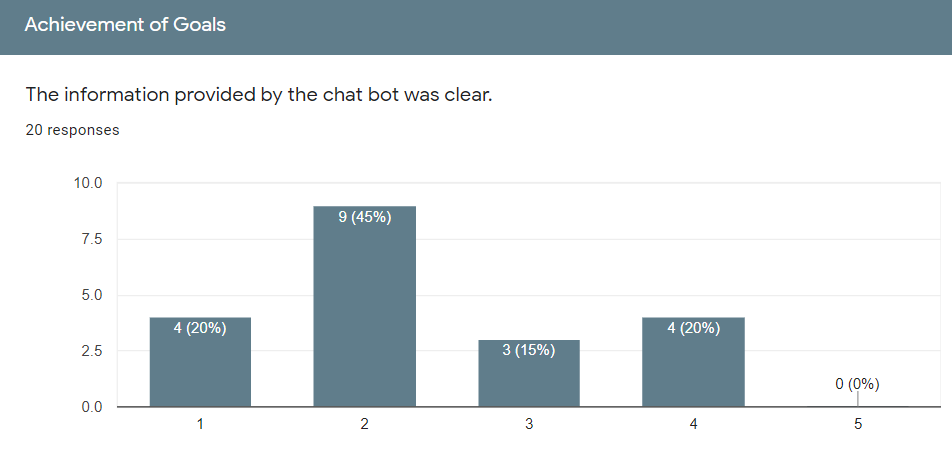
\includegraphics[width=0.9\textwidth]{img/Clear_Info.PNG}
%     \caption{Stats depicting about the information provided by the chat bot was clear}
%     \label{fig:clearInfo}
% \end{figure}
\\~\\
For the second statement, 10(50\%) disagreed with it which tells that for them the provided information was complete. Whilst 7(35\%) were unable to make any decision about it. This is something can not be ignored. It can happen due to various reasons: (i) due to lack of concentration (ii) misinterpretation of information or instructions (iii) chatbot responded falsely and a reason for it could be a weakly trained Rasa's NLU due to limited training data as already mentioned before. But still, 50\% answered that the information was complete, so there are high chances that the reason lies somewhere between (i) and (ii). Visuals have been shown in Figure \ref{fig:achievGoals}.

% \begin{figure}[!h]
%     \centering
%     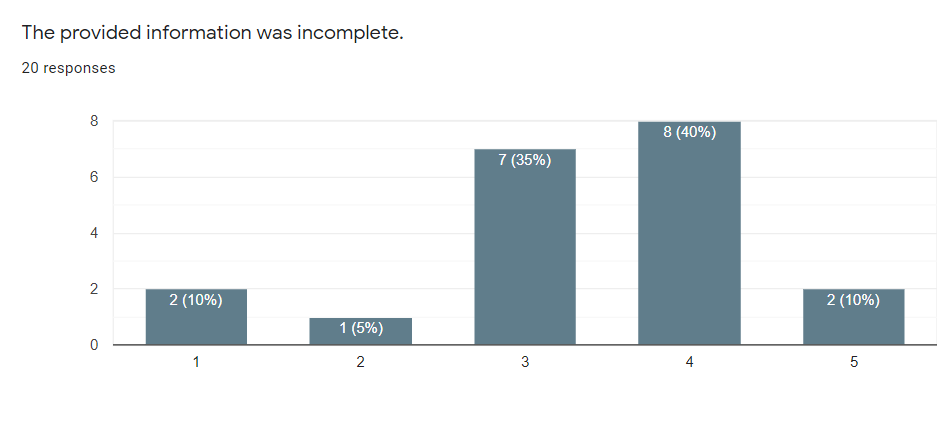
\includegraphics[width=0.9\textwidth]{img/Incomp_Info.PNG}
%     \caption{Stats depicting about the provided information was incomplete}
%     \label{fig:incompInfo}
% \end{figure}
\\~\\
Moving to what has been concluded from the third statement seems to be something positive. As 12(60\%) of the participants agreed upon the efficient interaction with the chatbot. Moreover, 4(20\%) failed to decide about it and only other remaining 4(20\%) disagreed with it. Refer to Figure \ref{fig:achievGoals} for better understanding by visuals.

% \begin{figure}[!h]
%     \centering
%     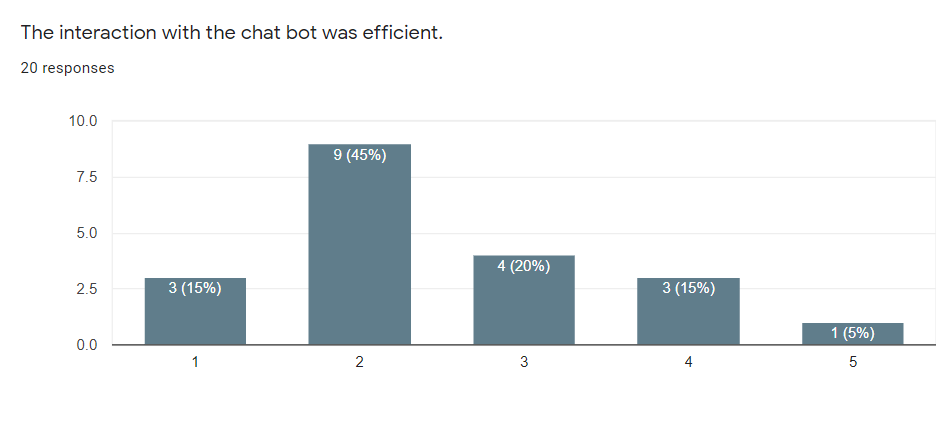
\includegraphics[width=0.9\textwidth]{img/Efficient_Inter.PNG}
%     \caption{Stats depicting about the interaction with the chat bot was efficient}
%     \label{fig:effInt}
% \end{figure}
\\~\\
Lastly, forth statement stats are a bit disappointing. According to only 6(30\%) users, the chatbot was reliable. On the contrary, 8(40\%) declared it unreliable, and the remaining 6(30\%) failed to take any decision about it. The possible reason for its unreliability could be its inability to respond to the user for all of his/her queries. And it happened due to limited data provided for training and also the demo chatbot was designed for limited use cases. To design a fully loaded chatbot that can reply to the user for any of his/her utterances, a lot of training data and processing is required and within limited time and resources, it was not possible. But, it could be done in the future. See Figure \ref{fig:achievGoals} for better visualization of the results.

% \begin{figure}[!h]
%     \centering
%     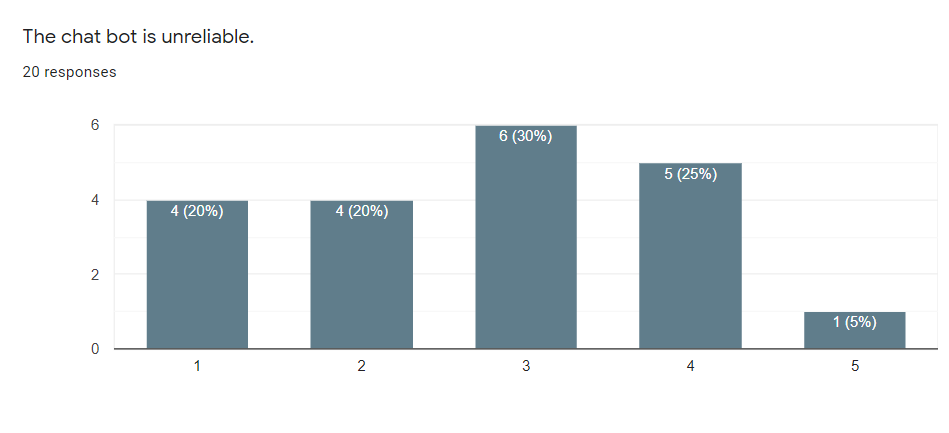
\includegraphics[width=0.9\textwidth]{img/Unreli_Bot.PNG}
%     \caption{Stats depicting about the chat bot is unreliable}
%     \label{fig:unreliBot}
% \end{figure}

\subsubsection*{Communication with the Chat Bot}
The purpose of this section was to collect the user's opinion that how was the communication with the chatbot. It consisted of the following three questions:
\begin{enumerate}
    \item The chatbot understood my messages well.
    \item I always knew what to say to the chatbot.
    \item The interaction with the chatbot sounded natural.
\end{enumerate}
Graphical representation for the detailed analysis and comparison of the results for these statements has been shown in Figure \ref{fig:communwithBot}.

\begin{figure}[!h]
    \centering
    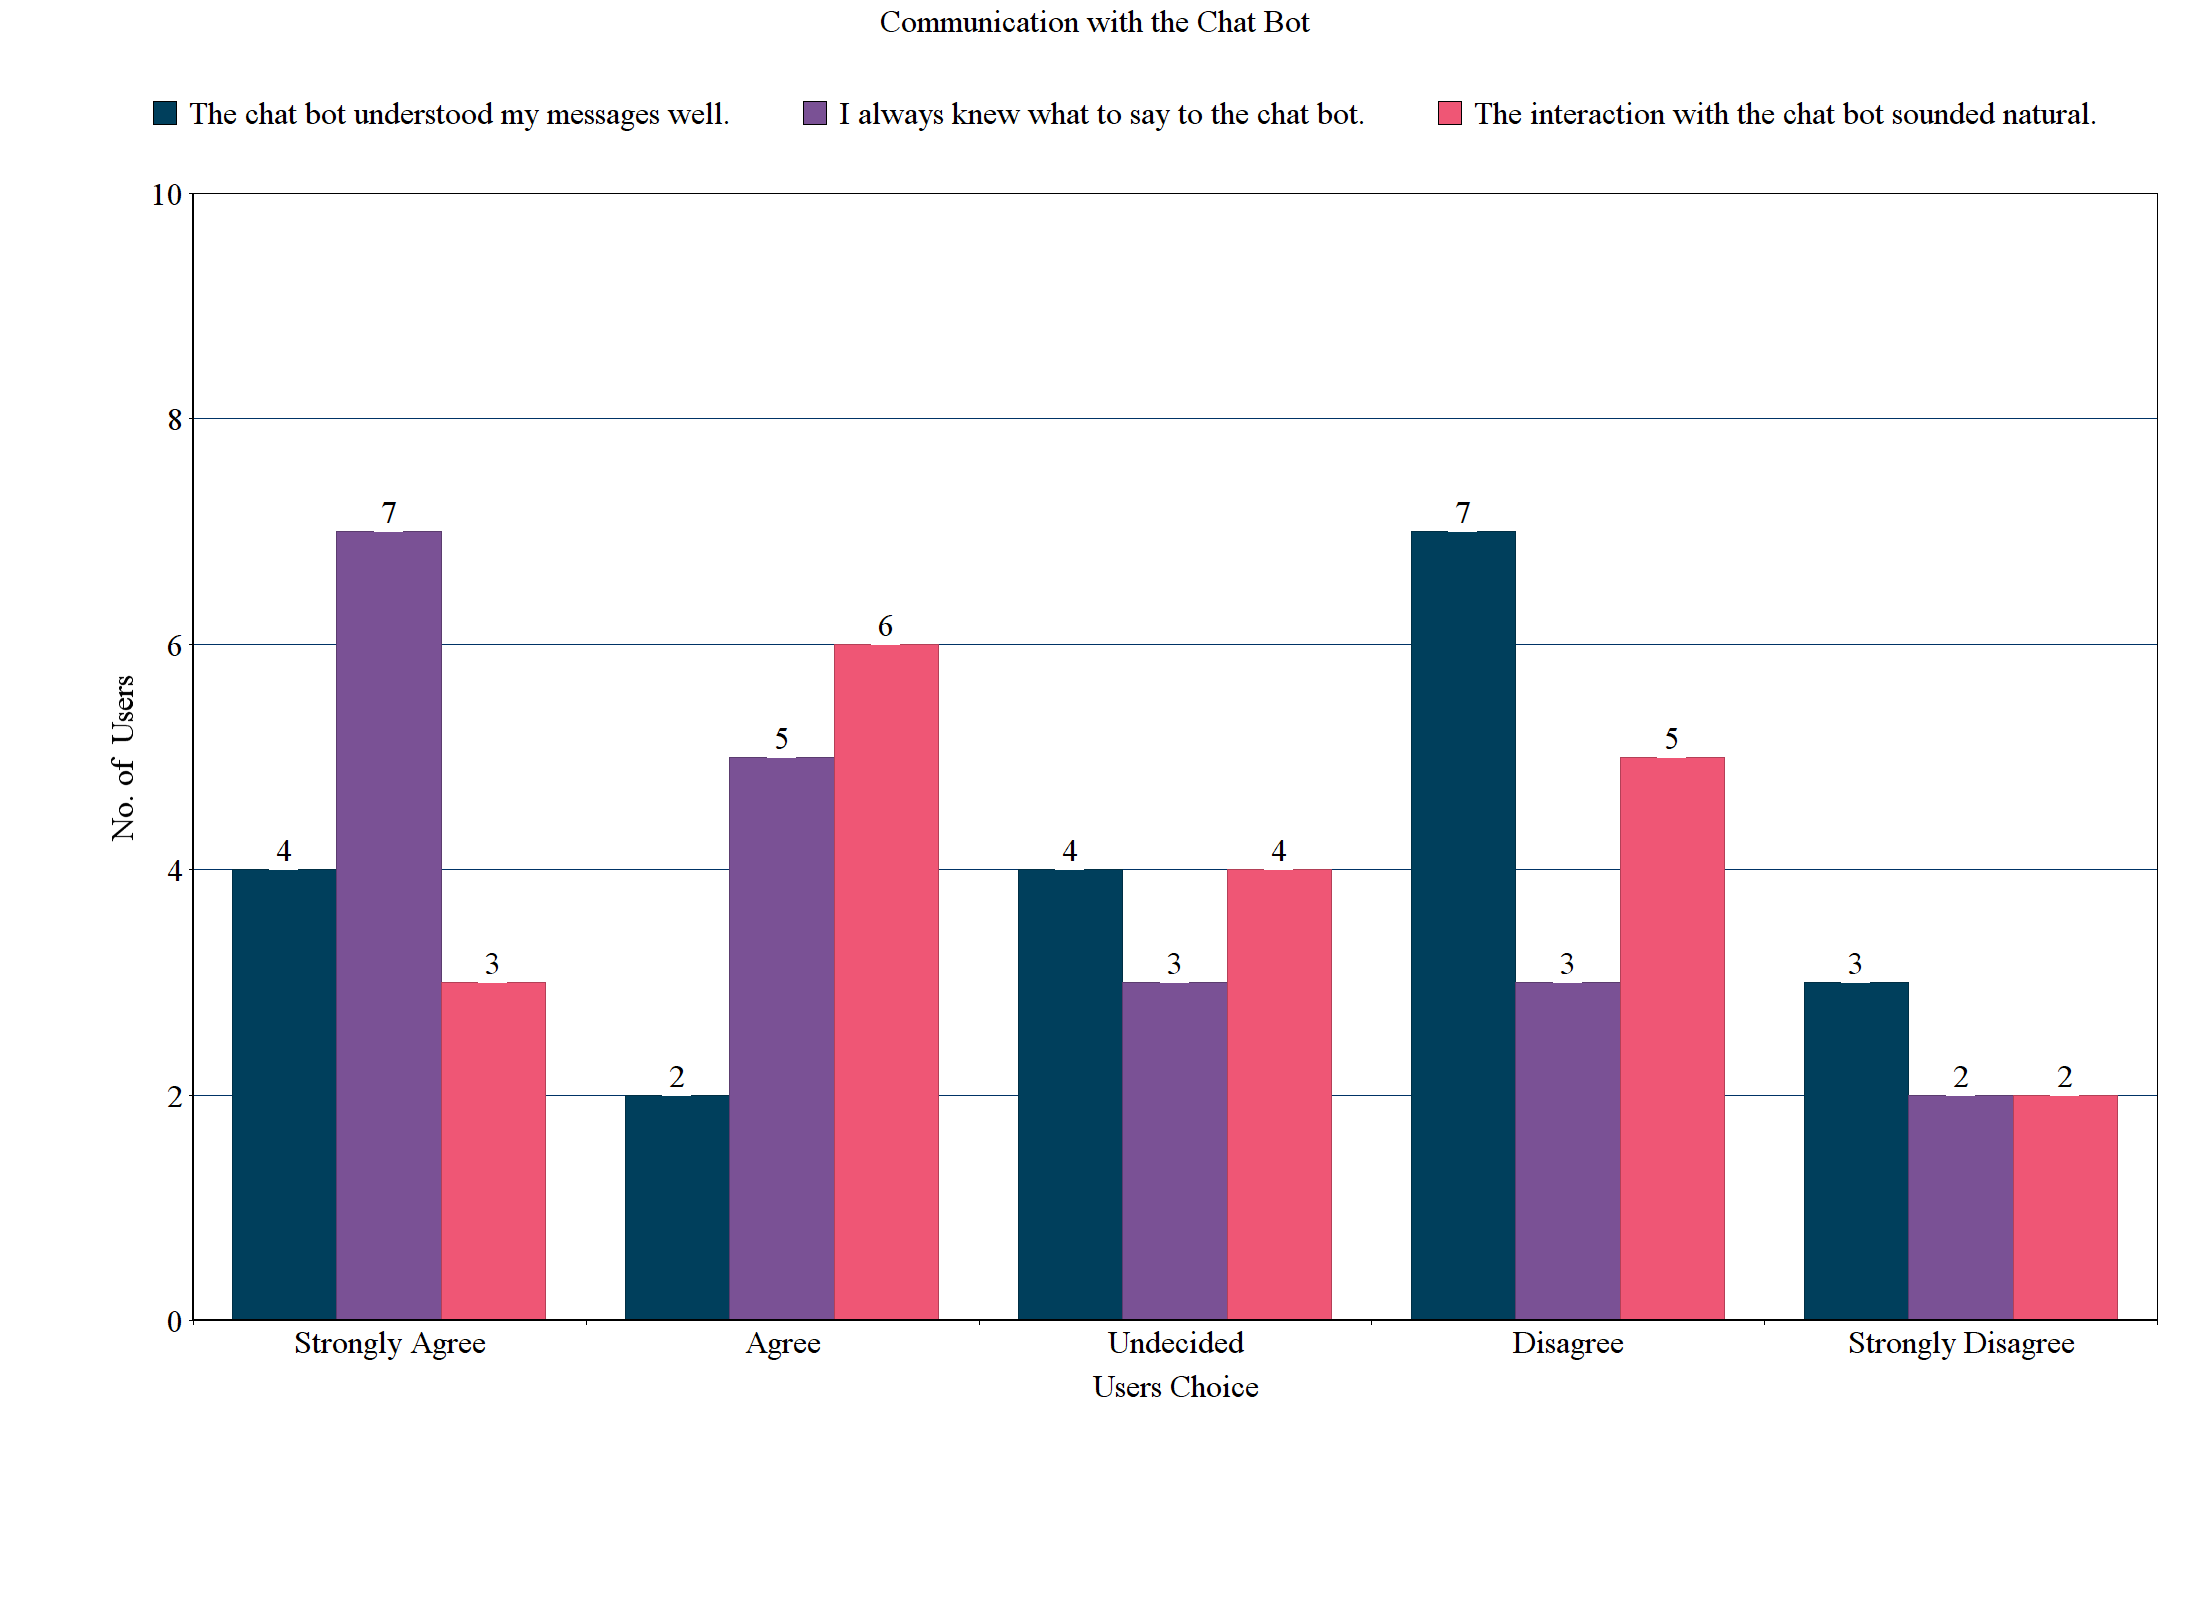
\includegraphics[width=0.9\textwidth]{img/Communication_with_the_Chat_Bot_Updated.png}
    \caption{Graphical representation of results collected for the users communication with the chat bot.}
    \label{fig:communwithBot}
\end{figure}
\\~\\
As extracted from graphical representation in Figure \ref{fig:communwithBot} that the total 10(50\%) of the participants disagreed with the statement that the chatbot understood their messages well. And 4(20\%) out of the remaining 10 were not able to decide about it. Remaining 6(30\%) answered positively with it. A majority disagreed with the statement and a reason could be the chatbot responded incorrectly. And it could be due to a problem with natural language understanding. It has been observed while testing that NLU was detecting wrong intents for the inputted utterances. The possible justification for it could be the limited training data used for learning as already mentioned in Section \ref{sec:expchatbot}. And the intents used in training have been displayed in Appendix \ref{appen:traindatastats}.

% \begin{figure}[!h]
%     \centering
%     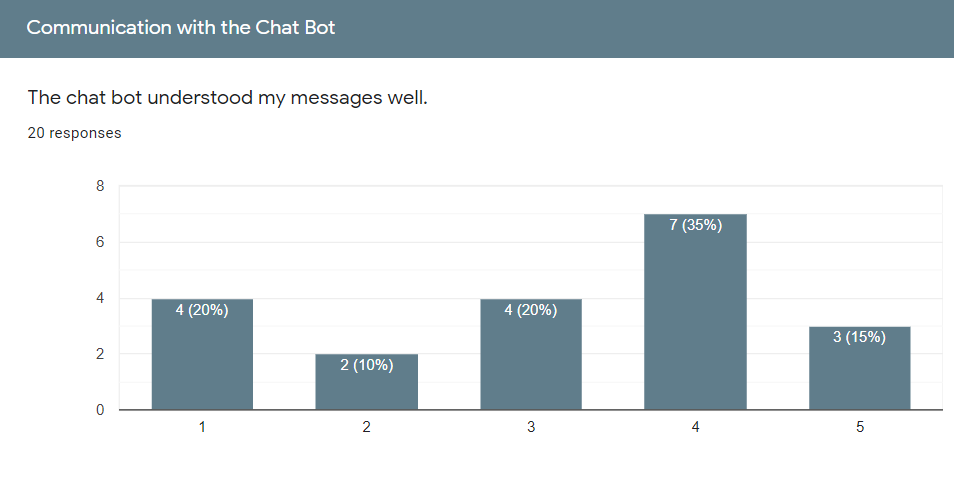
\includegraphics[width=0.9\textwidth]{img/Underst_Well.PNG}
%     \caption{Responses for the statement that the chat bot understood messages well.}
%     \label{fig:understWell}
% \end{figure}
\\~\\
Coming towards the next statement from Figure \ref{fig:communwithBot}, 12(60\%) of the users agreed that they always knew what to reply or ask the chatbot. Other than those, 3(15\%) failed to make any decision about it, and the remaining 5(25\%) disagreed with it. 
% Results have been displayed in the Figure .
% \begin{figure}[!h]
%     \centering
%     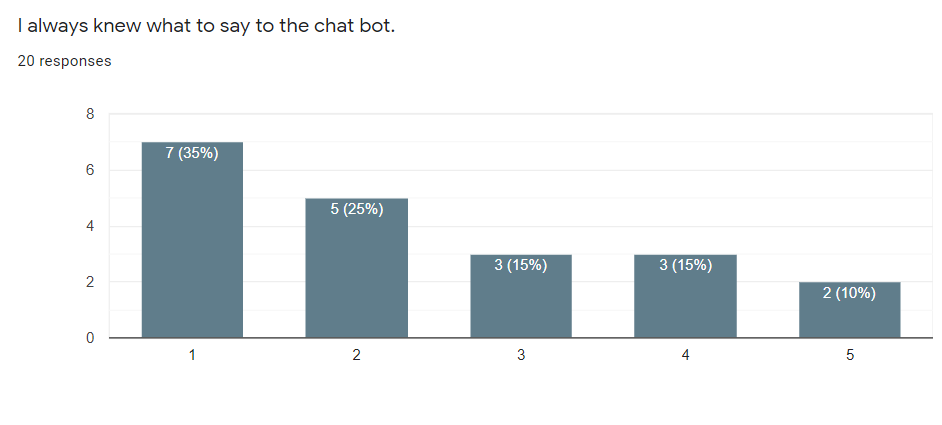
\includegraphics[width=0.9\textwidth]{img/Say_to_Bot.PNG}
%     \caption{Responses for the statement that the user always knew what to say to the chat bot.}
%     \label{fig:saytoBot}
% \end{figure}
\\~\\
Responses for the third statement from Figure \ref{fig:communwithBot} showed that 9(45\%) participants felt communication as natural. Out of the other 11, only 4(20\%) failed to decide about it. Along with that remaining 7(35\%) showed disagreement with it. And the reason could be the wrong intent detection by NLU. It has been observed through the information collected using a log file. Secondly, manually fed responses could also be a reason for it as every time it has to select from a fixed number of answers.
% For visuals, kindly have a look in to the Figure .
% \begin{figure}[!h]
%     \centering
%     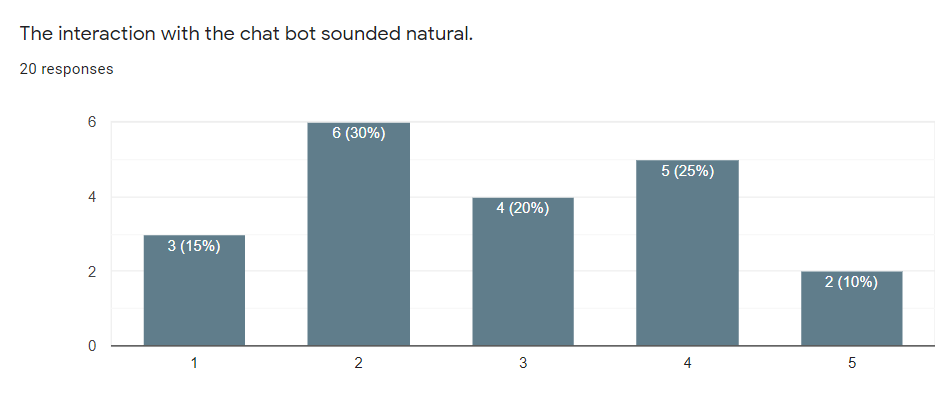
\includegraphics[width=0.9\textwidth]{img/Natural_Inter.PNG}
%     \caption{Responses for the statement that the interaction with the chat bot sounded natural.}
%     \label{fig:naturalInter}
% \end{figure}

\subsubsection*{Behaviour of the Chat Bot}
The intention behind adding this section to the questionnaire was to detect the behavior of the chatbot with the user. It consisted of the seven questions answered by the user on the scale of agreement or disagreement as stated below: 
\begin{enumerate}
    \item The chatbot responded too slowly.
    \item The chatbot is friendly.
    \item The chatbot didn't always meet my expectations.
    \item I didn't always know what answer the chatbot is expecting from me.
    \item The chatbot made many errors.
    \item I was able to recover easily from errors. (only in case of errors).
    \item The chatbot behaved cooperatively.
\end{enumerate}
Graphical representation for the detailed analysis and comparison of the results for these statements has been shown in Figure \ref{fig:behavofBot}.

\begin{figure}[!h]
    \centering
    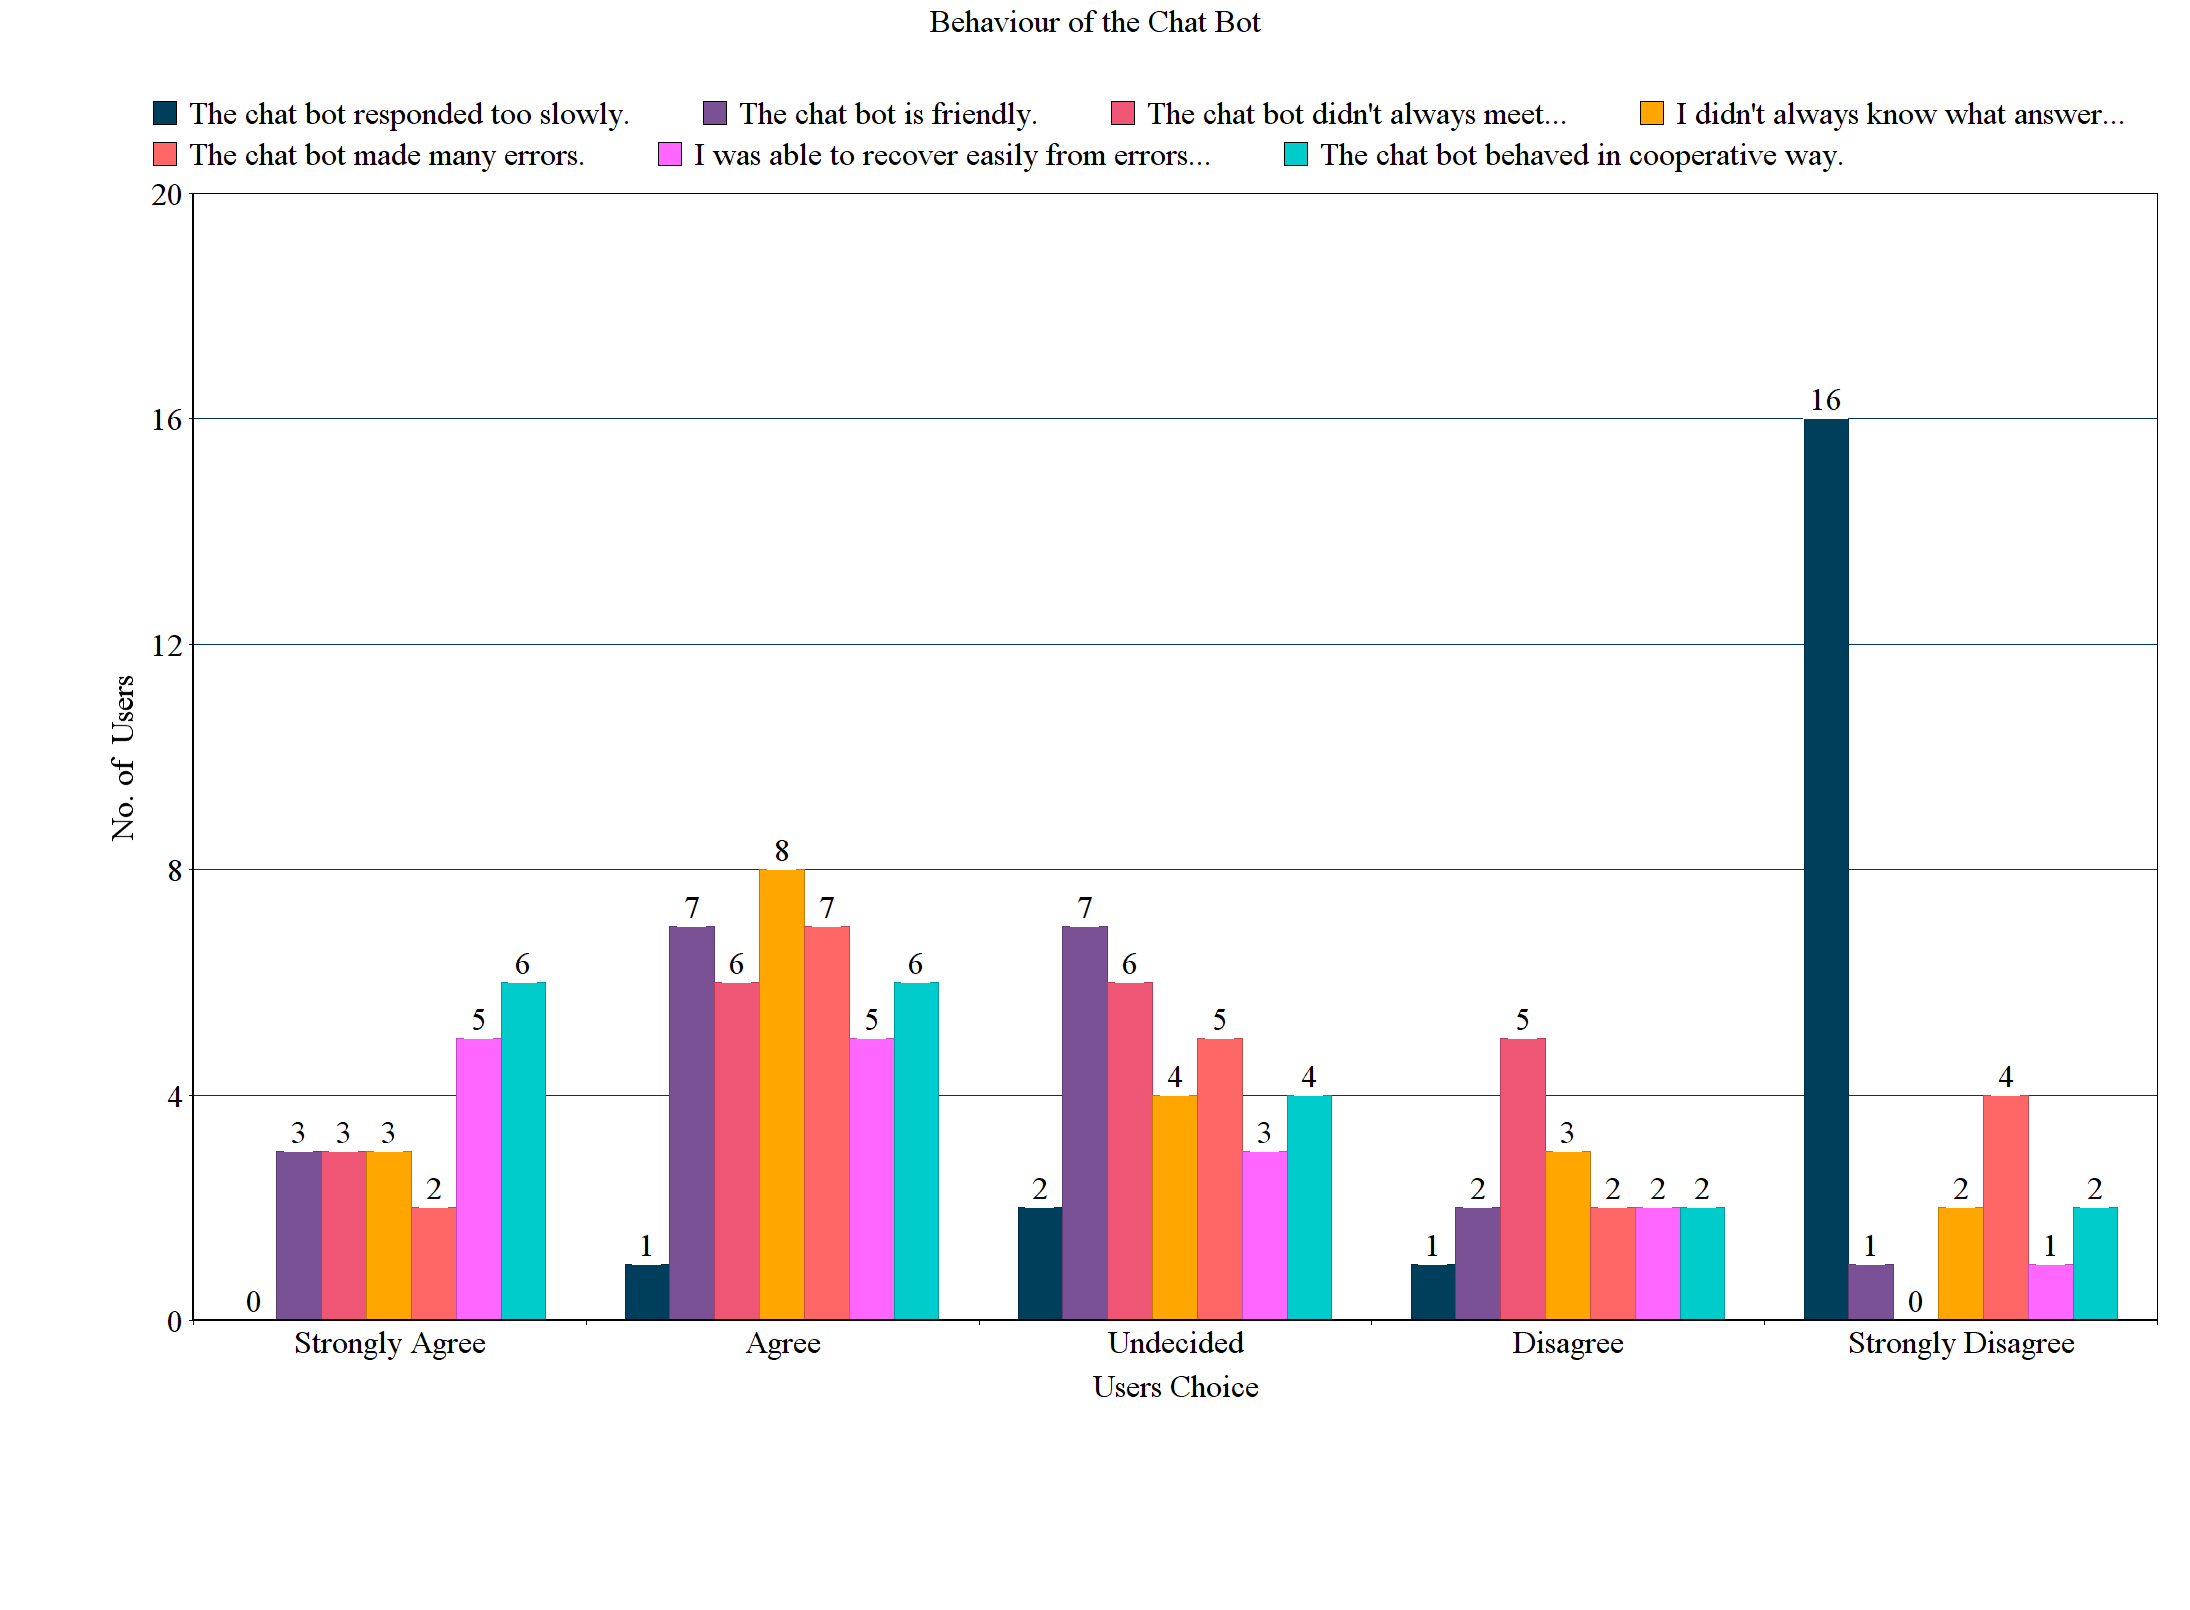
\includegraphics[width=0.9\textwidth]{img/Behaviour_of_the_Chat_Bot_Updated.png}
    \caption{Graphical representation of results collected for the behaviour of the chatbot.}
    \label{fig:behavofBot}
\end{figure}
\\~\\
Analyzing the results for this section's initial statement, 16(80\%) strongly disagreed with it. Whereas, another 1(5\%) also negated the statement which makes the number total 17(85\%) who portrayed that the responding speed for the chatbot was fast enough as shown in Figure \ref{fig:behavofBot}. 

% \begin{figure}[!h]
%     \centering
%     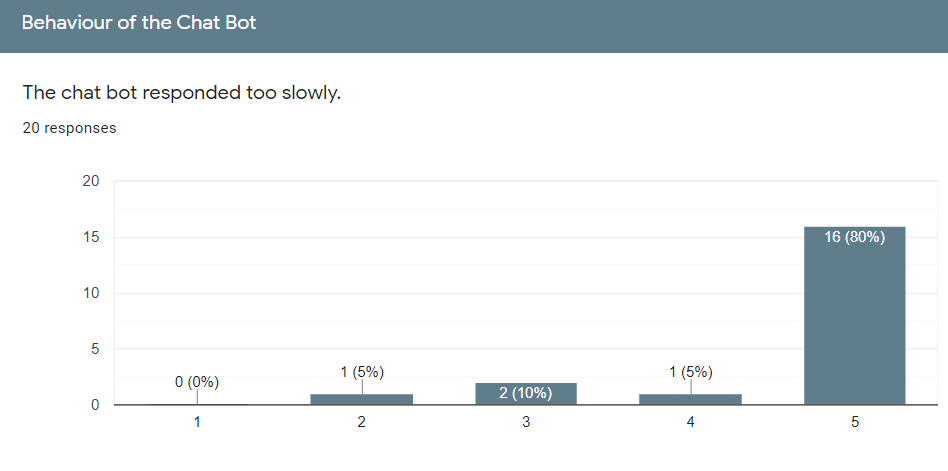
\includegraphics[width=0.9\textwidth]{img/Response_Speed.PNG}
%     \caption{Result about the chat bot's response speed}
%     \label{fig:respSpeed}
% \end{figure}
\\~\\
Secondly, 10(50\%) rated the chatbot as friendly. While 7(35\%) other respondents were unable to come up with any decision about it as displayed in Figure \ref{fig:behavofBot}. It could be due to the reason that different persons have their perception of friendliness. Also, the demo topic included detective bot. So, it was meant to respond with straight forward statements. Which could be felt a bit offensive some times depending upon the user's mood and nature. 

% \begin{figure}[!h]
%     \centering
%     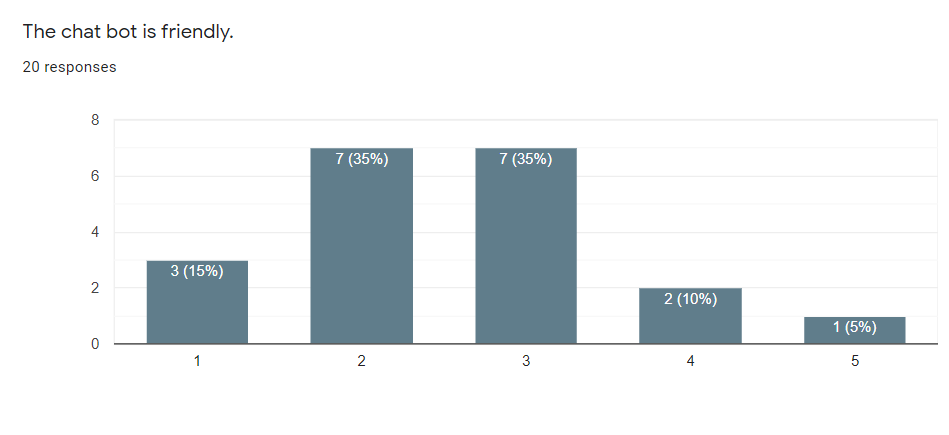
\includegraphics[width=0.9\textwidth]{img/Friendly_Chatbot.PNG}
%     \caption{Result about the chat bot's friendliness}
%     \label{fig:friendlyBot}
% \end{figure}
\\~\\
Thirdly, the chatbot didn't meet the expectations for 9(45\%) of the participants. Additionally, the other 6(30\%) were failed to determine it and only 5(25\%) stated that it fulfilled their expectations and can be visualized in Figure \ref{fig:behavofBot}. So it can be concluded from it that the chatbot failed to impress the users by its behavior. The possible reason for it might be the same as the statement in the last section that the chatbot didn't understand the messages well or the users found it harsh or offensive.

% \begin{figure}[!h]
%     \centering
%     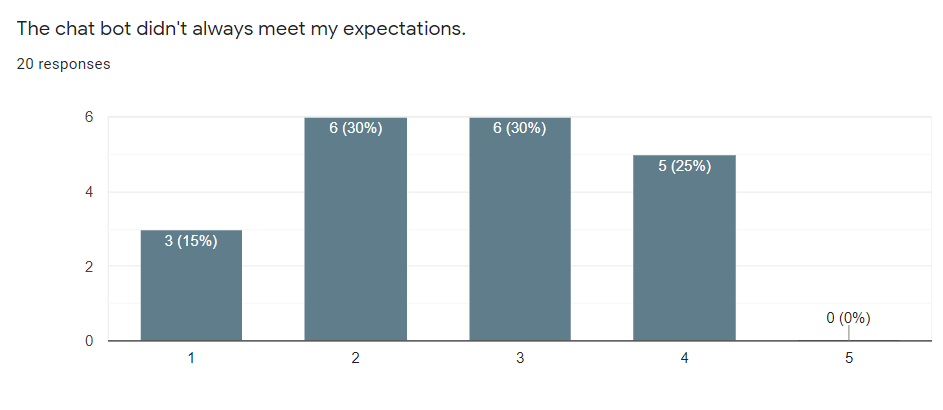
\includegraphics[width=0.9\textwidth]{img/Chatbot_Expect.PNG}
%     \caption{Result for the expectations from the chat bot}
%     \label{fig:botExpec}
% \end{figure}
\\~\\
Reviewing the results for the fourth statement, 11(55\%) of the respondents showed agreement with the statement that they didn't always know what answer was the chatbot expecting from them as displayed in the Figure \ref{fig:behavofBot}. It could be due to the limitation of the training data as the chatbot was just trained for limited intents but the users were provided with free choice to ask anything from the chatbot. 

% \begin{figure}[!h]
%     \centering
%     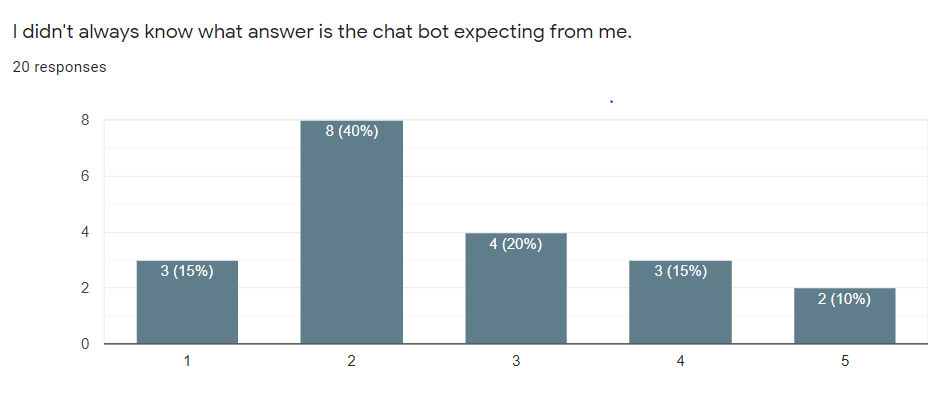
\includegraphics[width=0.9\textwidth]{img/Answer_Expect.PNG}
%     \caption{Result for the users knowledge about the chatbot's expectation}
%     \label{fig:ansExpec}
% \end{figure}
\\~\\
Checking with the participants' opinion about errors made by the chatbot and recovery from them, 9(45\%) stated that chatbot made errors. While 6(30\%) negated it and the remaining 5(25\%) were unable to decide about it. But the positive point about the chatbot was, out of those users who faced the error or unable to decide about it during a chat, 10 of them were able to recover easily from the error. In addition to that, 12(60\%) of the participants rated the chatbot as cooperative. On the contrary, just 4(20\%) marked it as uncooperative as shown in Figure \ref{fig:behavofBot}.

% \begin{figure}[!h]
%     \centering
%     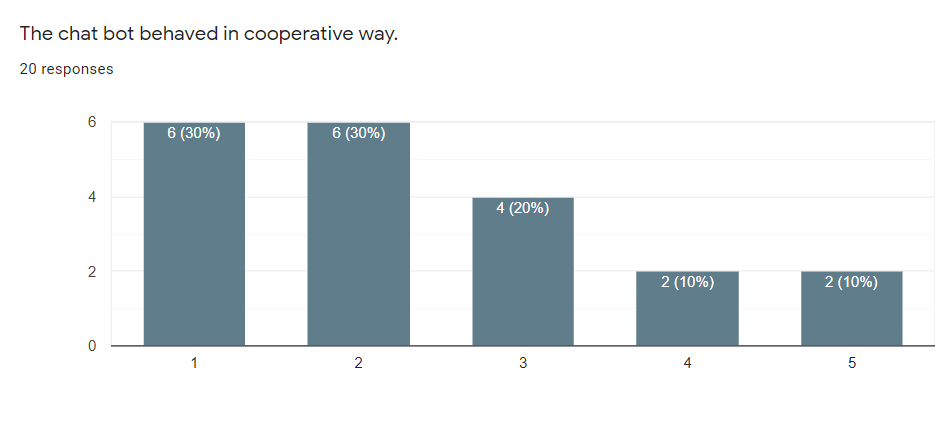
\includegraphics[width=0.9\textwidth]{img/Cooperative_Chatbot.PNG}
%     \caption{Result about the the chatbot's cooperativity}
%     \label{fig:cooperBot}
% \end{figure}

\subsubsection*{Dialogue Assessment}
This part of the survey was added to judge the design of the dialogue according to the users' perspective. A total of six questions were asked by the participants for completion of the purpose.
\begin{enumerate}
    \item I easily lost track of where I am in an interaction with the chatbot.
    \item The dialogue was bumpy.
    \item I was able to direct the conversation as desired.
    \item I felt in control of the interaction with the chatbot.
    \item The dialogue quickly led to the desired goal.
    \item The dialogue parts were evenly distributed between me and the chatbot.
\end{enumerate}
Graphical representation for the detailed analysis and comparison of the results for these questions has been displayed in Figure \ref{fig:dialogAssess}.

\begin{figure}[!h]
    \centering
    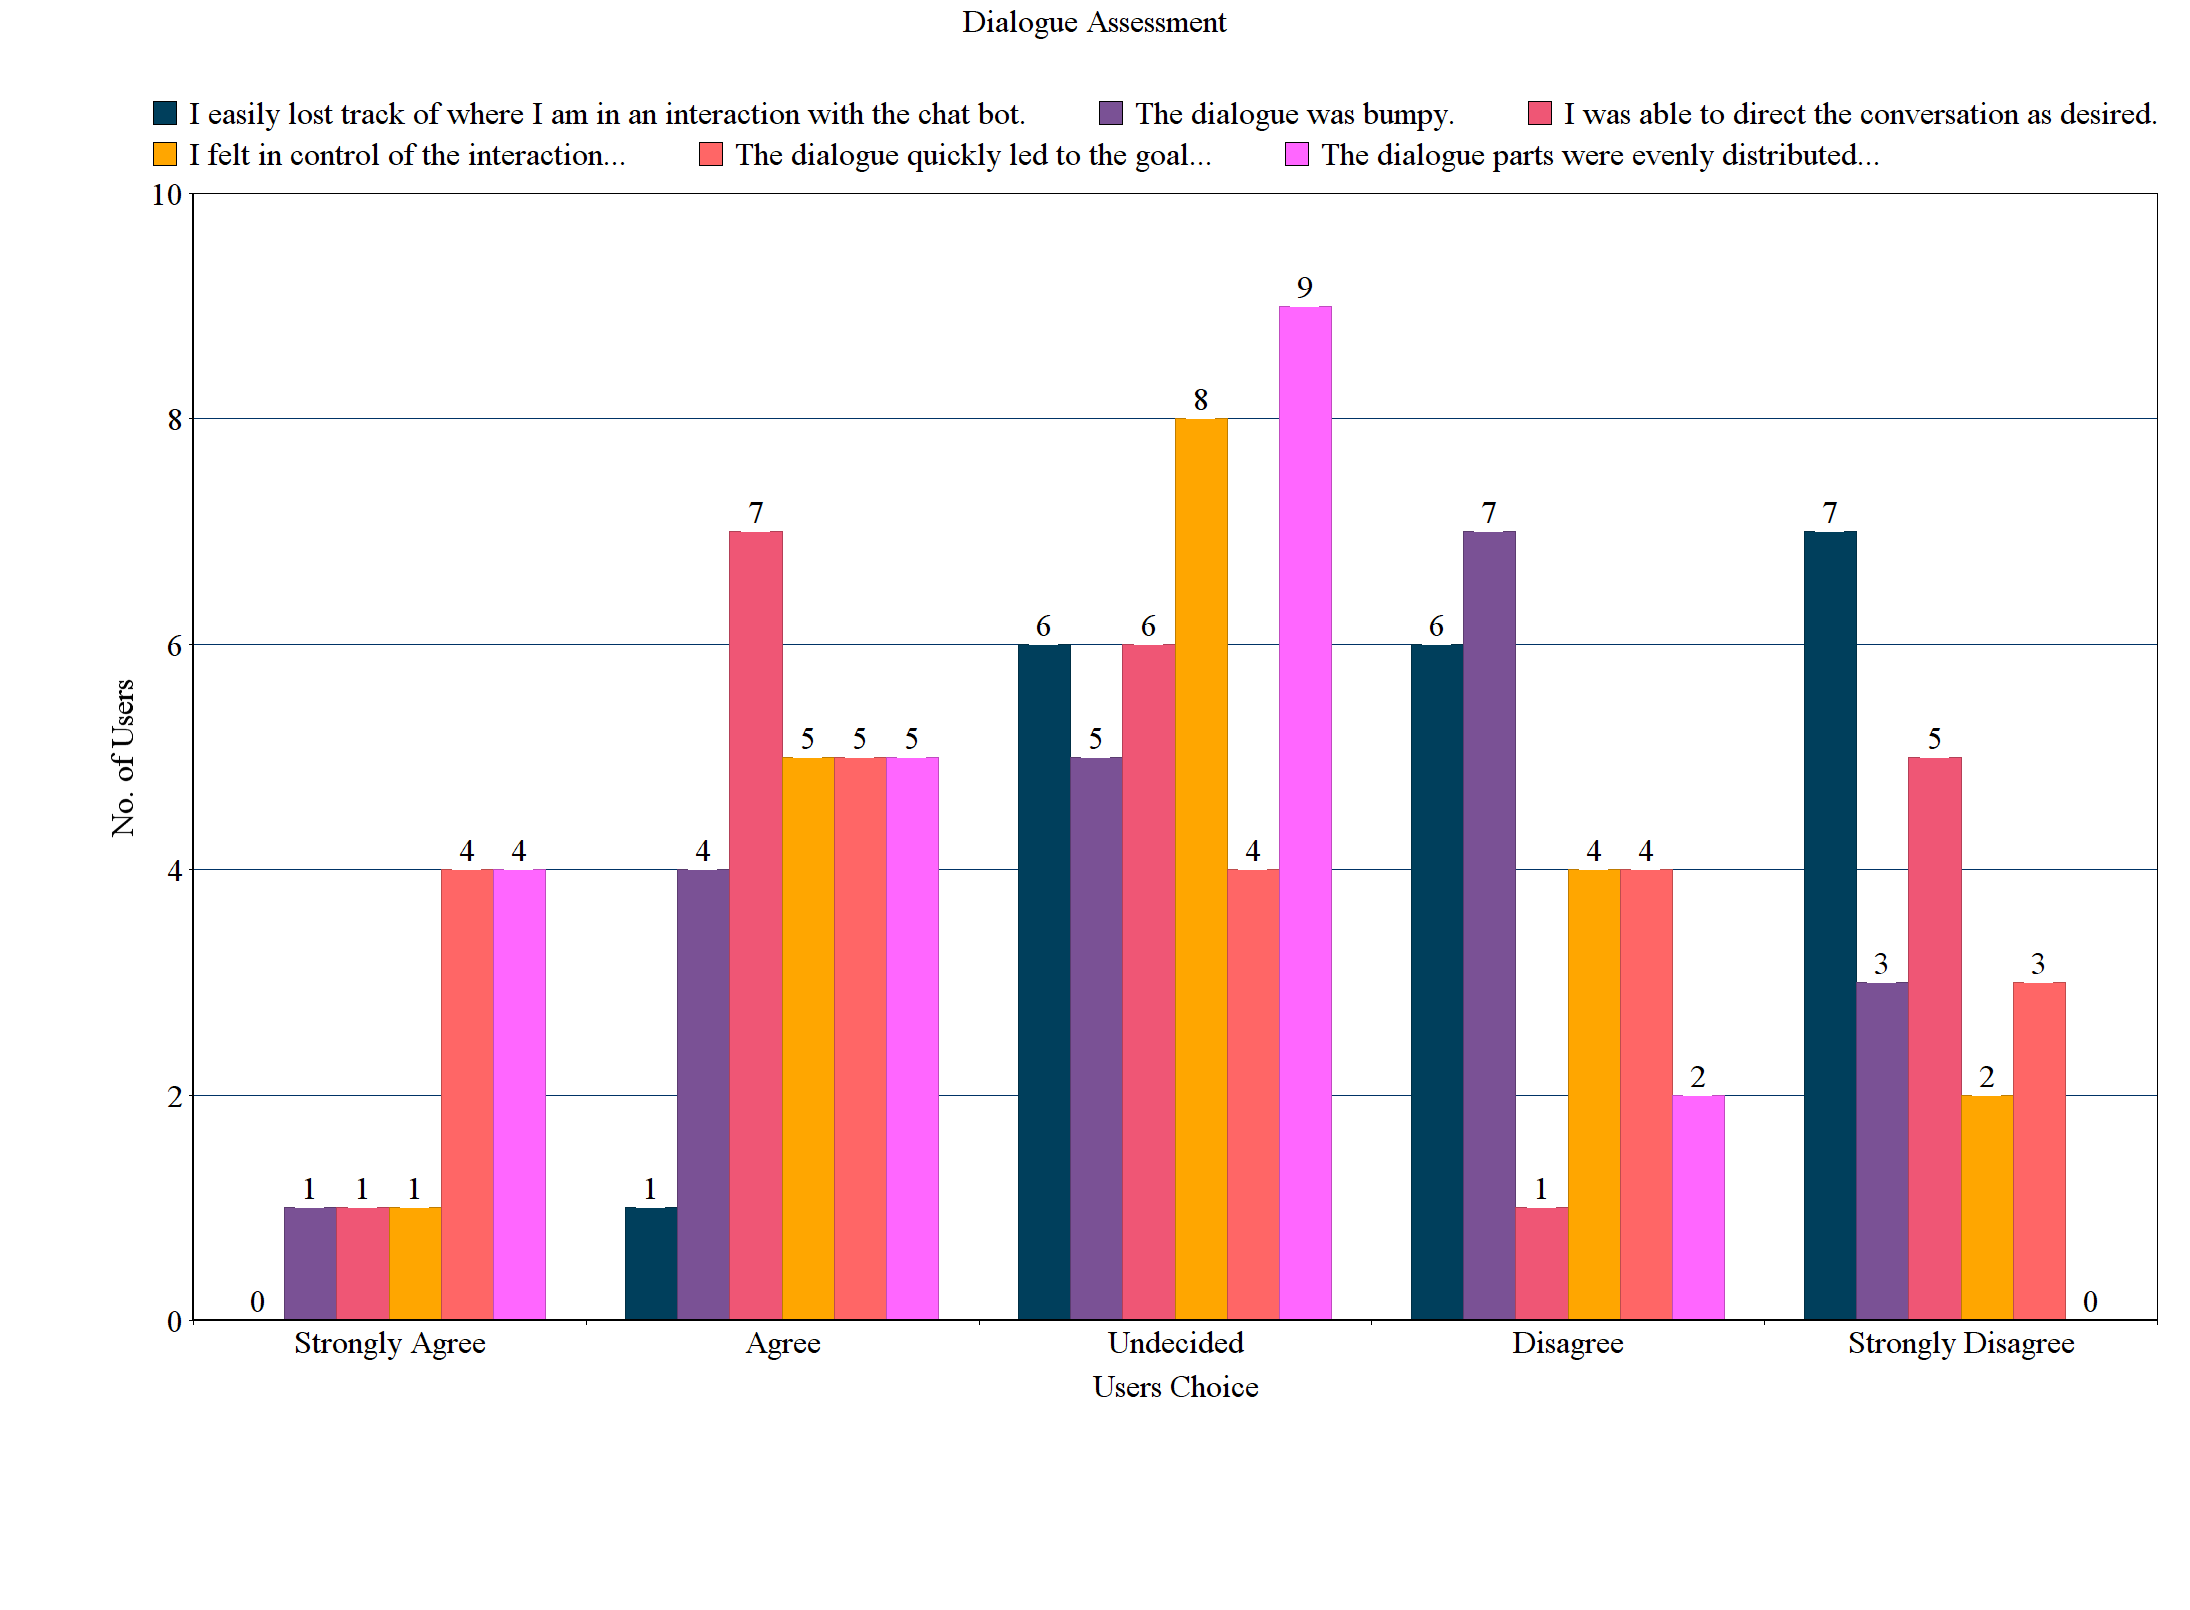
\includegraphics[width=0.9\textwidth]{img/Dialogue_Assessment_Updated.png}
    \caption{Graphical representation of results collected for the dialogue assessment.}
    \label{fig:dialogAssess}
\end{figure}
\\~\\
As plotted in Figure \ref{fig:dialogAssess} that 7(35\%) strongly disagreed while 6(30\%) simply disagreed with the statement that they lost the track during the communication with the chatbot. On the other hand, 6(30\%) were unable to make any decision and only 1(5\%) just agreed with it. So it can be concluded from the result analysis that maintaining a state for each module concerning each user has been appeared useful and effective.

% \begin{figure}[!h]
%     \centering
%     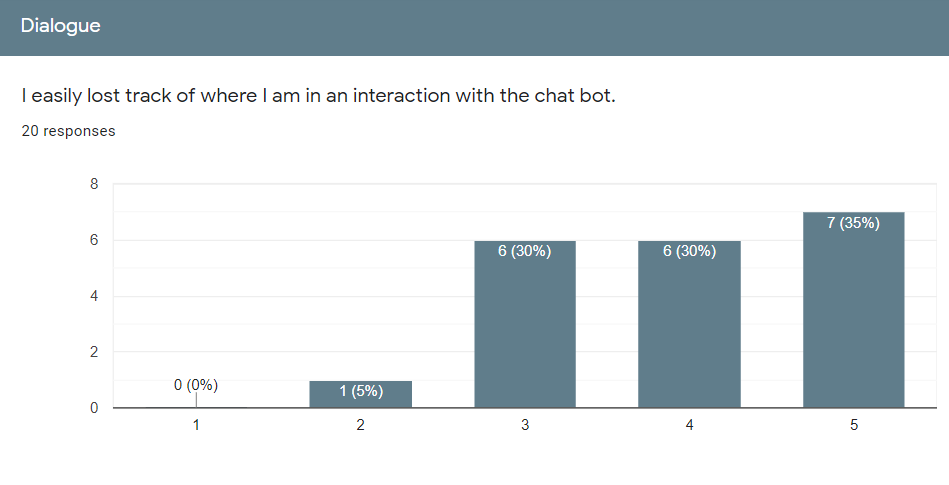
\includegraphics[width=0.9\textwidth]{img/Lost_Track.PNG}
%     \caption{Result for users lost track during interaction with the chatbot}
%     \label{fig:lostTrack}
% \end{figure}
\\~\\
After analyzing the results from Figure \ref{fig:dialogAssess}, it is not wrong to say that the dialogue was smooth and communication between the users and the chatbot was comfortable and consistent. 10(50\%) of the participants showed disagreement with the statement that the dialogue was bumpy. Contrarily, only half of it that is 5(25\%) just find it unstable. This means by using the modular architecture a stable and smooth dialogue can be designed.

% \begin{figure}[!h]
%     \centering
%     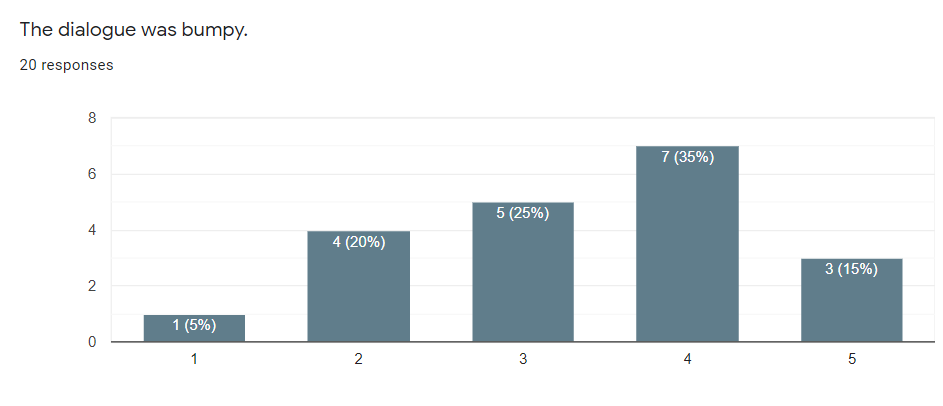
\includegraphics[width=0.9\textwidth]{img/Bumpy_Dialog.PNG}
%     \caption{Result reflecting users opinion about bumpy dialogue}
%     \label{fig:bumpDialo}
% \end{figure}
\\~\\
Nextly, as presented in Figure \ref{fig:dialogAssess} that 8(40\%) of the participants were able to direct the conversation according to their desires. On the other hand, 6(30\%) out of the remaining 12 were unable to drive it according to their wish. And the left out 6(30\%) answered as undecided. And yet again the ratio of the respondents who were able to direct the conversation as desired appeared to be greater than the ones who were not able to do it.

% \begin{figure}[!h]
%     \centering
%     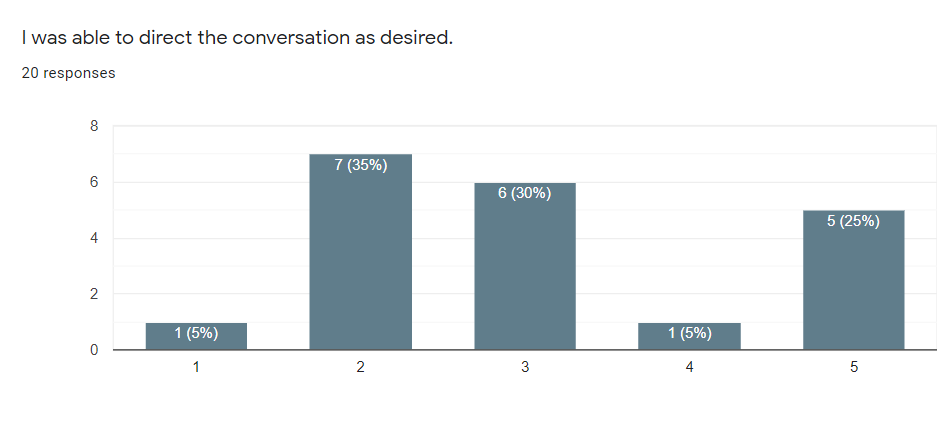
\includegraphics[width=0.9\textwidth]{img/Desired_Conv.PNG}
%     \caption{Result reflecting users opinion about desired conversation}
%     \label{fig:desiredConv}
% \end{figure}
\\~\\
As shown in Figure \ref{fig:dialogAssess}, that the number of participants who agreed and disagreed with the statement that they felt in control of the conversation with the chatbot is the same and that is 6(30\%) for both categories. And remaining 8(40\%) were not able to decide about it. Now it is something alarming, as in this case, a possible reason could be the topic of the demo chatbot. As I designed the detective chatbot and it was designed in a way to be a bit strict and commanding. 

% \begin{figure}[!h]
%     \centering
%     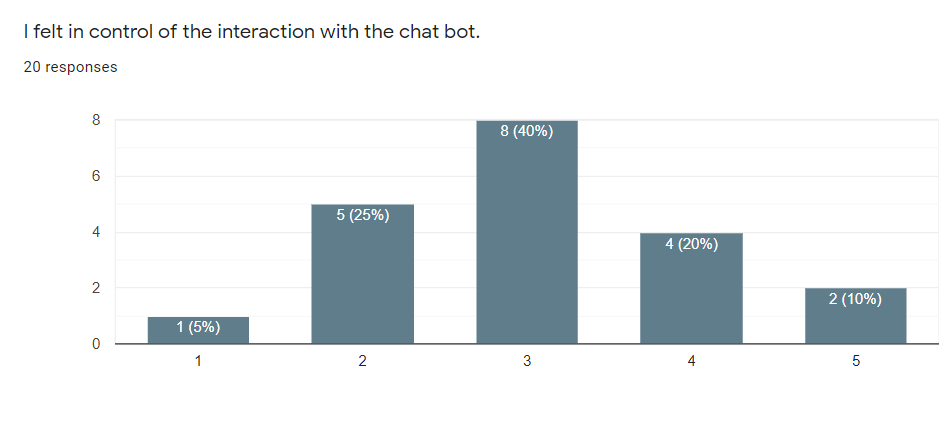
\includegraphics[width=0.9\textwidth]{img/Chatbot_Control.PNG}
%     \caption{Result reflecting users opinion whether they felt that the chat was controlled by the chatbot}
%     \label{fig:chatbotControl}
% \end{figure}
\\~\\
According to Figure \ref{fig:dialogAssess}, 9(45\%) answered that the dialogue quickly led to the desired goal which refers to the fact that the detective game was designed in such manner that the user should be able to reach the final goal as quickly as possible. But also 7(35\%) disagreed with it and the cause behind it could be the wrong intent detection as the user typed in something else but NLU recognized it differently due to which chatbot responded with some unrelated statement.

% \begin{figure}[!h]
%     \centering
%     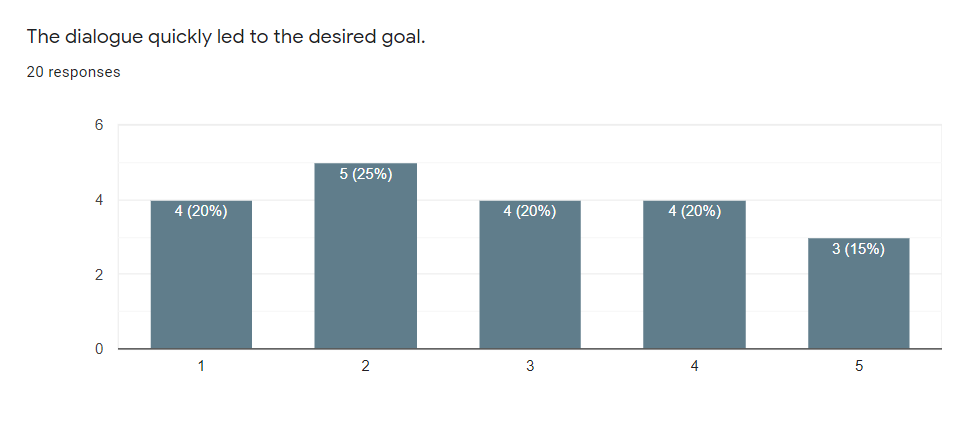
\includegraphics[width=0.9\textwidth]{img/Quick_Goal.PNG}
%     \caption{Result reflecting users opinion about the dialogue quickly led to the goal}
%     \label{fig:quickGoal}
% \end{figure}
\\~\\
Referring to Figure \ref{fig:dialogAssess}, 9(45\%) of the people who took part in the study agreed with a statement that dialogue parts were equally distributed between them and chatbot. Whereas other 9(45\%) were leave it undecided and only 2(10\%) disagreed with it.

% \begin{figure}[!h]
%     \centering
%     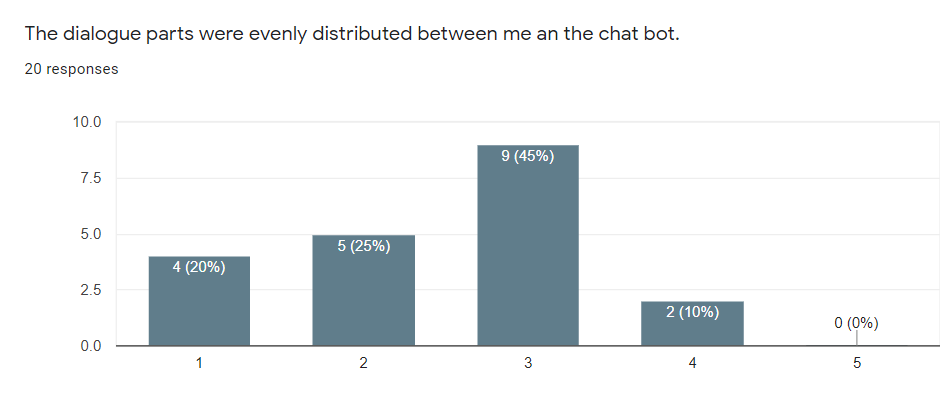
\includegraphics[width=0.9\textwidth]{img/Even_Parts.PNG}
%     \caption{Result reflecting users opinion about the equal distribution of the dialogue parts}
%     \label{fig:evenDist}
% \end{figure}

\subsubsection*{Personal Experience and Impression}
This segment has been put to the questionnaire to collect users' experience and personal impressions about the chatbot. It also has been completed using a series of questions. 
\begin{enumerate}
    \item The interaction with the chatbot was pleasant.
    \item I felt relaxed.
    \item High level of concentration is required while using the chatbot.
    \item The interaction was fun.
    \item Overall, I am satisfied with the chatbot.
    \item I felt that the chatbot was smart enough to handle the message which was not lying in its scope.
    \item I felt that the chatbot guided me well to return to the actual topic when I tried to misguide it.
    \item It was easy for me to continue the chat without any reluctance.
    \item It was easy for me to understand the response of the chatbot.
    \item It took me too long to make the chatbot understand my message by using different terms in sentences.
\end{enumerate}
Graphical representation for the detailed analysis and comparison of the remarks for these assertions has been shown in Figure \ref{fig:persExpandImp}.

\begin{figure}[!h]
    \centering
    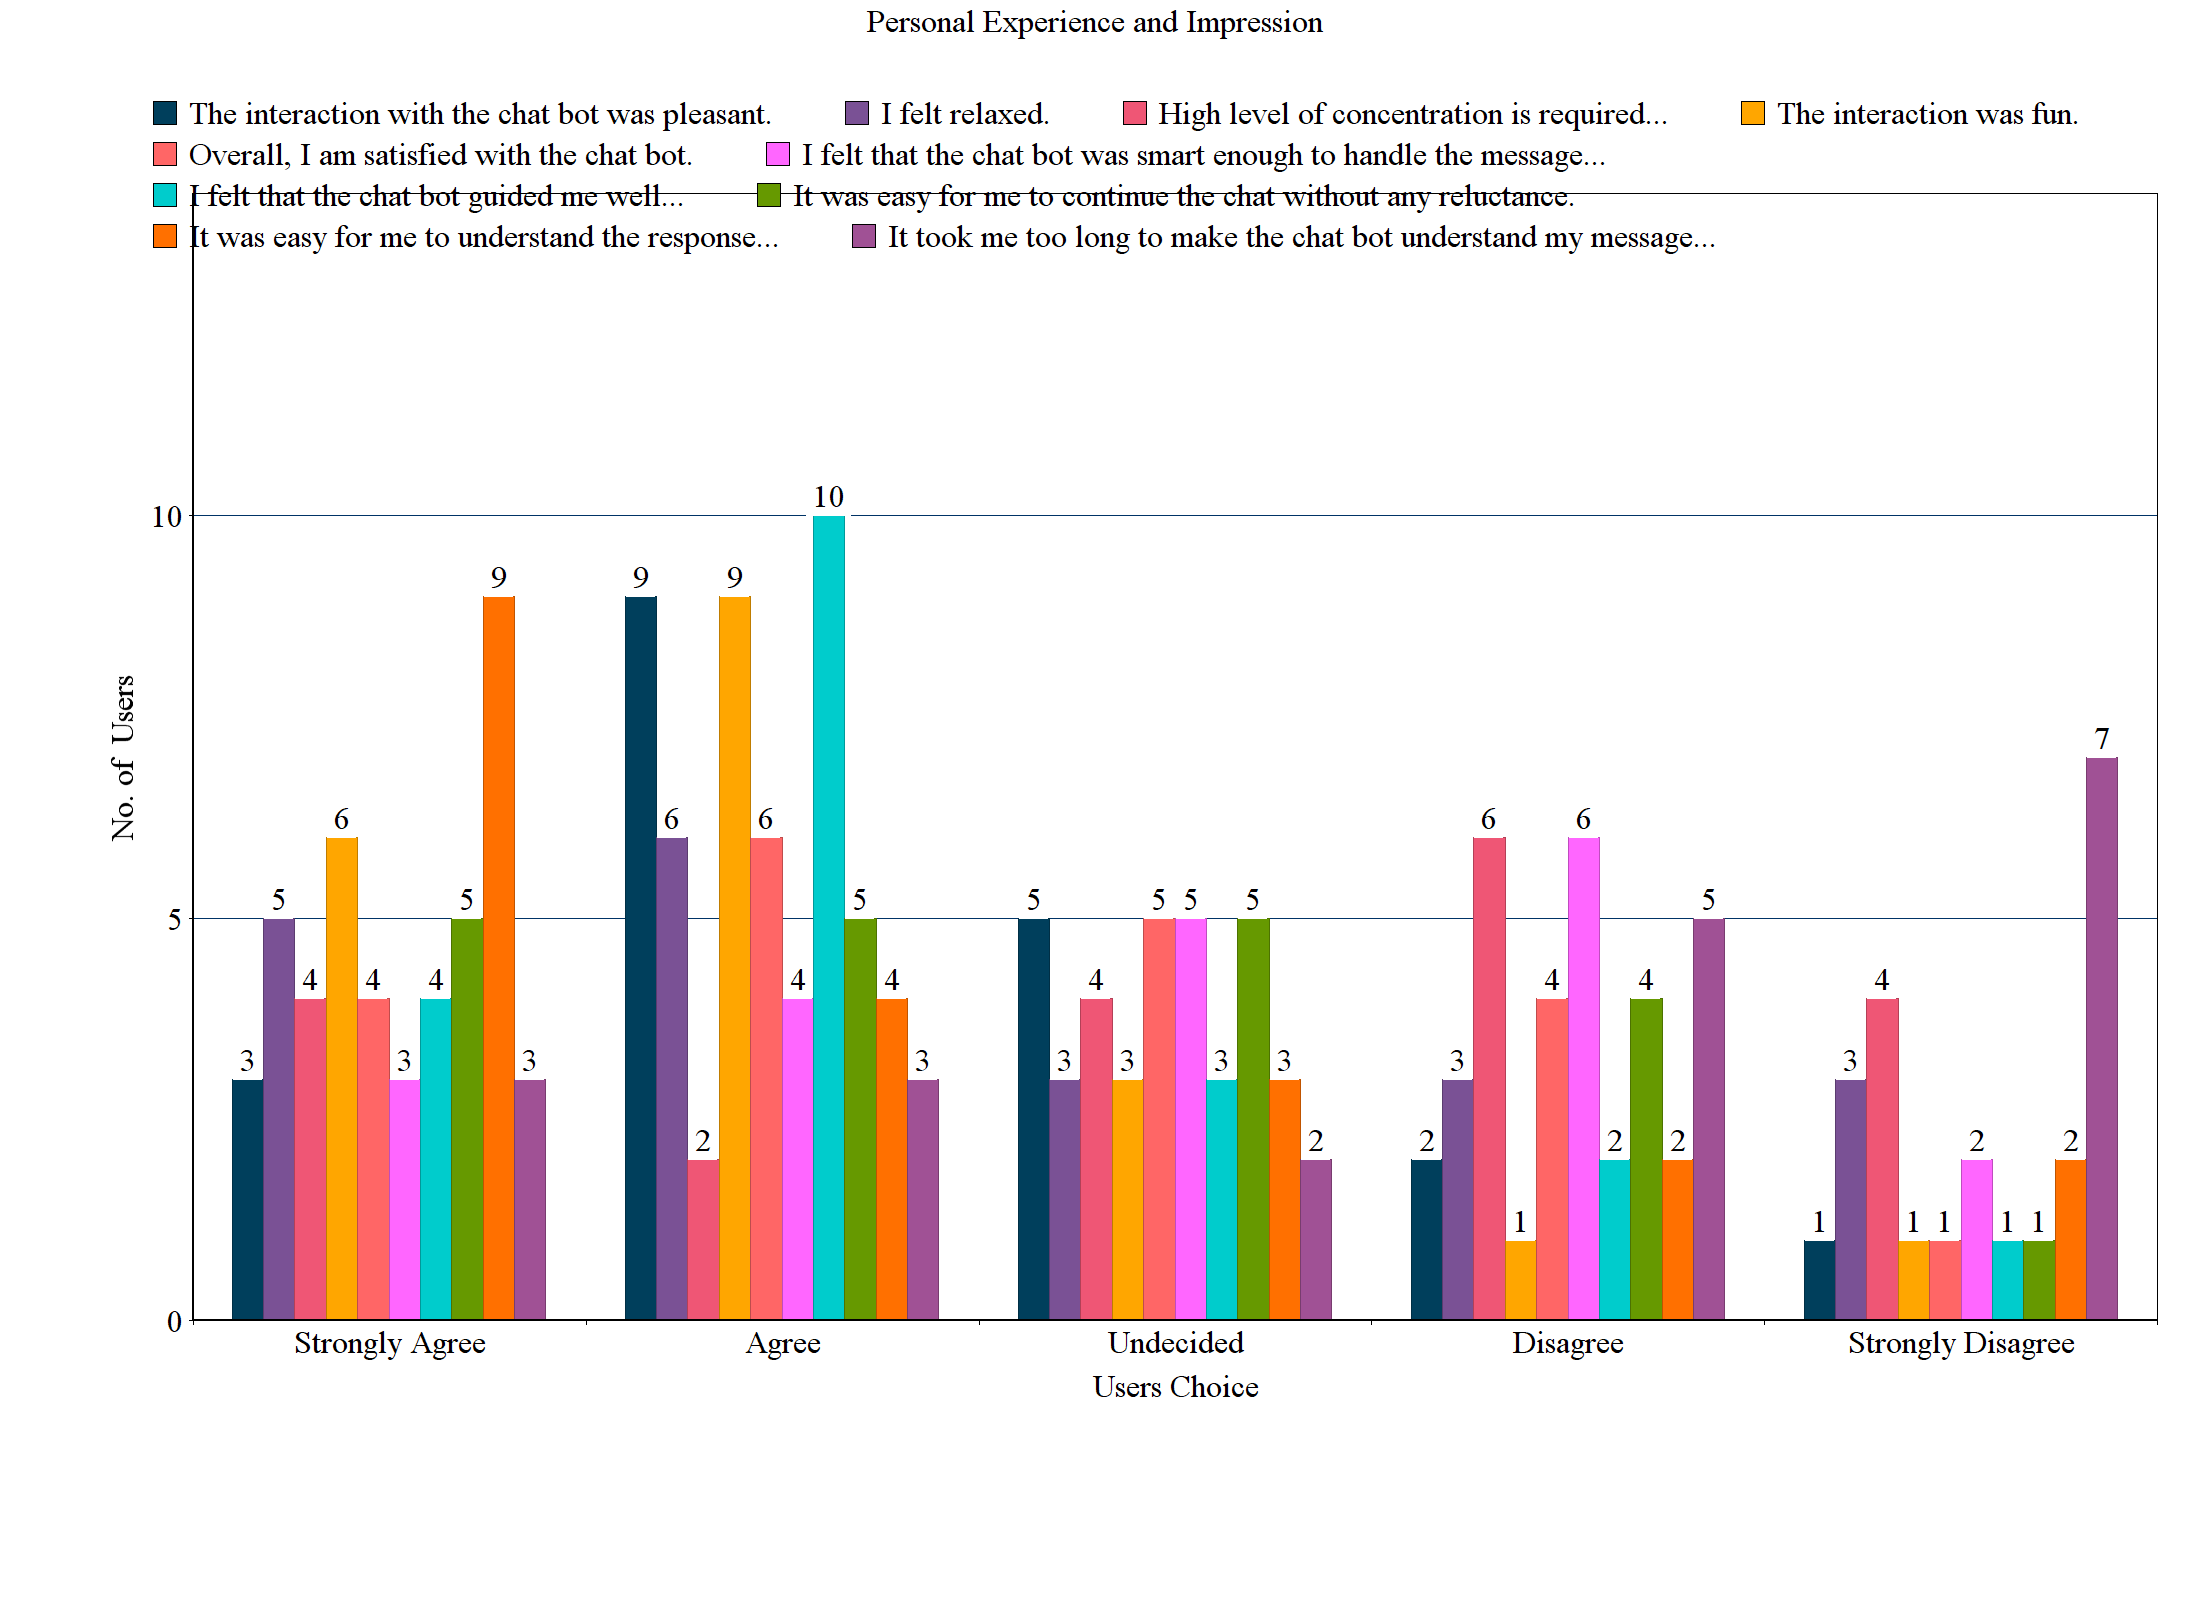
\includegraphics[width=0.9\textwidth]{img/Personal_Experience_and_Impression_Updated.png}
    \caption{Graphical representation of results collected for the users personal experience and impression.}
    \label{fig:persExpandImp}
\end{figure}
\\~\\
As presented in Figure \ref{fig:persExpandImp}, the majority of the participants i.e. 12(60\%) felt that the interaction with the chatbot was pleasant. It could be due to the reason that the user doesn't have to restart the chat whenever he/she wants to move to some different topic. The user was able to jump between different topics at any moment and can handle multiple topics at the same time without losing the state for the last topic. 
\\~\\
According to Figure \ref{fig:persExpandImp}, 11(55\%) respondents responded that they felt relaxed while having a conversation with the chatbot. It was something important to make sure that chatbot is not making someone feel tensed or bad about anything. Furthermore, 10(50\%) of the users also showed disagreement with the statement that a high level of concentration was required while using the chatbot. So, from this result, it can be concluded that the chatbot and the dialogue design was simple and also user friendly. Additionally, 15(75\%) of the users found the interaction as fun. It was also the main purpose of the Frankenbot to entertain the users instead of making them feel bored. So, this purpose also gets accomplished. 
\\~\\
After analyzing the result from Figure \ref{fig:persExpandImp} about the user satisfaction for the chatbot, it can be deduced that the majority of the users 10(50\%) felt satisfied with it. While 5(25\%) out of the other 10 left it undecided and the remaining 5(25\%) were not satisfied with it.
\\~\\
Nextly, as figured out from Figure \ref{fig:persExpandImp}, majority 8(40\%) of the participants disagreed that the chatbot was able to handle the messages well which were out of its scope. Whereas, 7(35\%) of the respondents agreed with it. By surveillance of the log file based on detected intents for user utterances, it has been observed that the wrongly recognized intent could be a reason for it. Otherwise, the framework has been tested in such a way that, if on each step an utterance is provided from training data and intent has been identified correctly then its performance was up to the mark. Secondly, it has been designed to handle such a scenario well as already explained in Chapter \ref{cha:chapter3} of this document. In addition to it, 14(70\%) of the respondents showed agreement to the statement that chatbot guided them well to return to the actual topic when they tried to misguide it. It makes the stance clear about the chatbot abilities that it contains the skills to well manage the messages which do not lie under its scope.
\\~\\
Moving to the next statement, 10(50\%) of the users agreed that they were able to continue the chat without any stoppage. It means the chatbot was working well for them as they wanted. The chatbot nor the user were reluctant to each other. It can also be concluded from this result that the dialogue was well structured and designed to perform smooth conversation without any objection or hesitation. Another important factor that can't be neglected is that the user should be able to understand the chatbot's response. So, 13(65\%) of the participants were able to do so. Which also marked this property as accomplished for the chatbot.
\\~\\
Lastly, 12(60\%) out of the total 20 participants negated the statement that it took them too long to make the chatbot understand their message by using different terms in sentences. It reflects that the information provided to the users was pretty much clear and also the guidance by the chatbot was enough for the user to enter the correct answer.

\subsubsection*{Usability}
This part of the survey has been added to gather the users' opinions about the chatbot's usefulness and whether it is easy to use or not. So, it has been judged based on what users have answered the following questions:
\begin{enumerate}
    \item The system is difficult to use.
    \item It is easy to learn to use the chatbot.
    \item The chatbot is too inflexible.
    \item I would like to use the chatbot again in the future.
    \item The chatbot operation was worthwhile.
\end{enumerate}
Graphical representation for the detailed analysis and comparison of the responses for these assertions has been shown in Figure \ref{fig:usabil}.

\begin{figure}[!h]
    \centering
    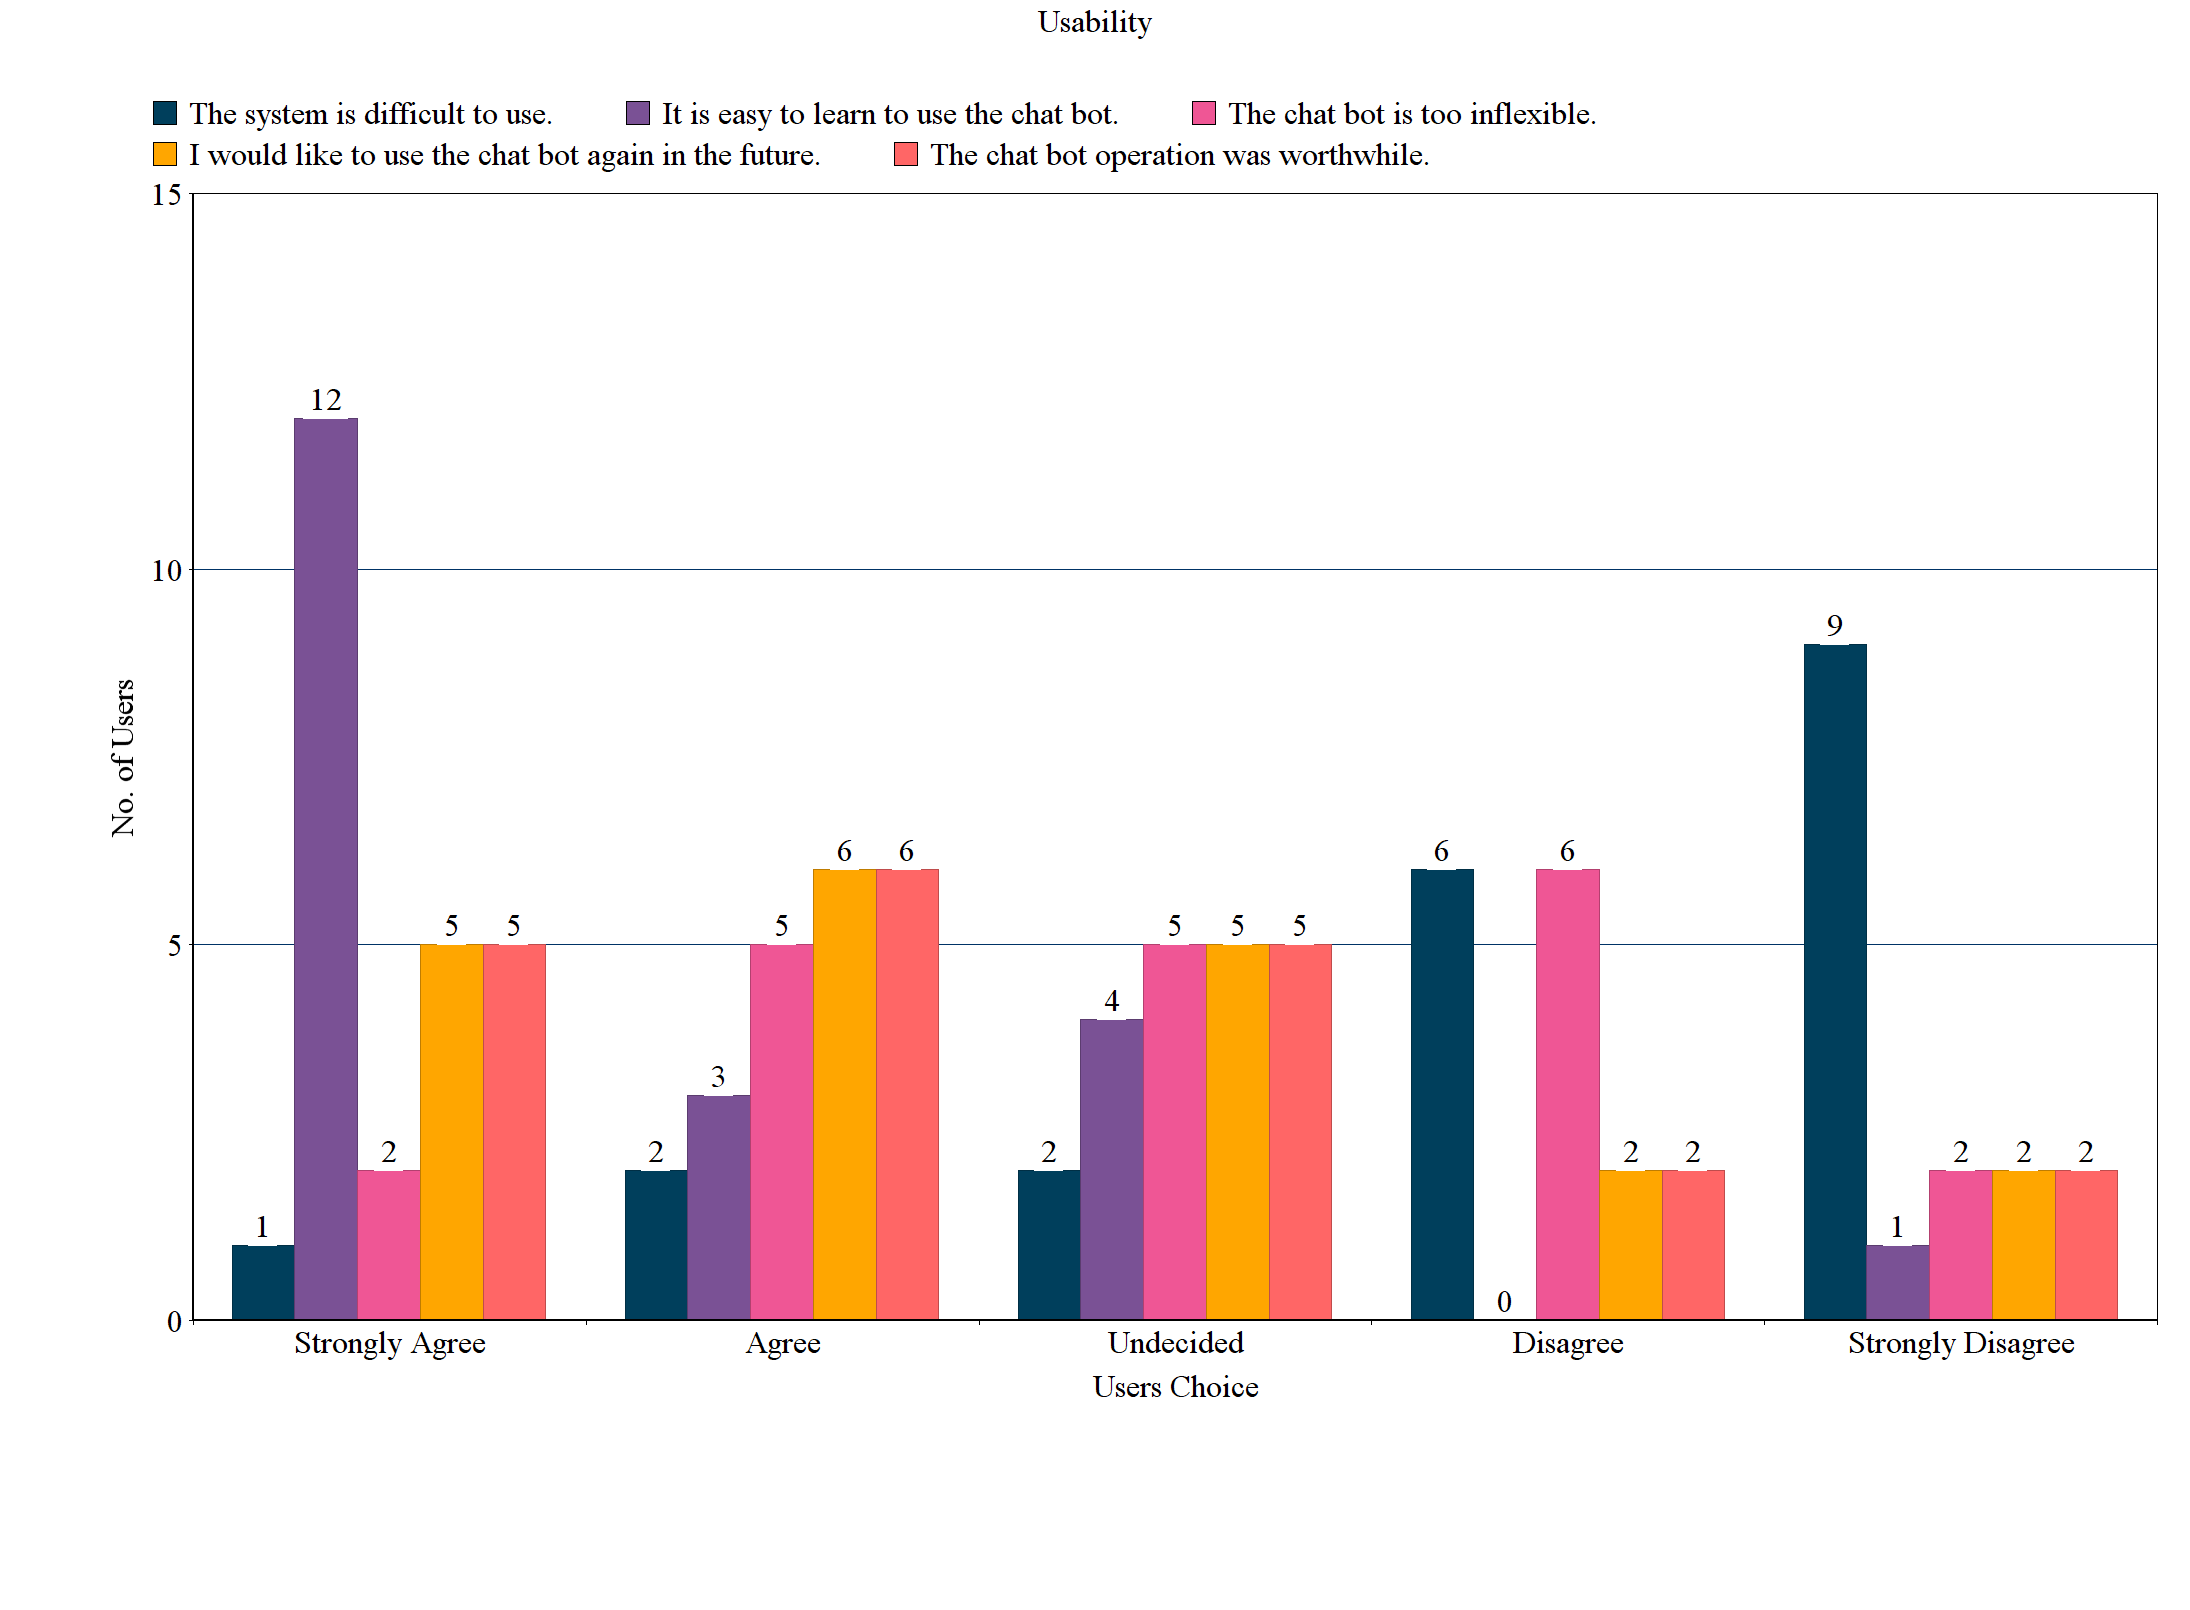
\includegraphics[width=0.9\textwidth]{img/Usability_Updated.png}
    \caption{Graphical representation of results collected for the chatbot's usability.}
    \label{fig:usabil}
\end{figure}
\\~\\
According to the result deduced from Figure \ref{fig:usabil}, 15(75\%) of the users contradicted with the statement that the chatbot was difficult to use. Which means the majority of the participants found it easy to use. Additionally, again the same amount of the respondents i.e. 15(75\%) discovered that it was easier to understand the chatbot. It could be due to several reasons like the information provided was enough, the chatbot's ability to guide the user, structured dialogue, and a good understanding of the chatbot's response by the user.
\\~\\
Furthermore, 8(40\%) of the respondents disagreed with the statement that chatbot was too inflexible. Whereas, 7(35\%) showed agreement on this statement. This mixed opinion of the users could be just because of the reason that the chatbot was designed in a way that it should guide the user to return to the actual topic instead of continuing the chat on any user's desired topic. As the chatbot has been trained using limited data, time, and resources. Once, it will undergo good training then one can easily make it work for all user utterances regardless of the specific topic.
\\~\\
In the end, the users were asked whether they want to use the chatbot again in the future. And 11(55\%) replied positively. Contrarily, only 4(20\%) responded negatively. Moreover, they were also asked to rate the chatbot's functioning whether it's worth the time and effort spent. And majority i.e. 11(55\%) of the participants agreed with it. On the other hand, only 4(20\%) of respondents disagreed with it.

\subsection{Evaluation via AttrakDiff}
AttrakDiff's single evaluation method\footnote{\url{http://www.attrakdiff.de/#tab-einsatz}} has been used to judge the chatbot based on the following qualities:
\begin{itemize}
    \item Hedonic quality (HQ), includes 14-word pairs which refer to the joy of use, emphasized stimulation, identification, and evocation generated by the system.
    \item Pragmatic quality (PQ), involves 7-word pairs that reflect the system's usefulness, efficiency, and how easy is it to use.
    \item Attractiveness (ATT), it is also comprised of 7 items that are being used to judge the system's pleasantness and how catchy is it according to the user's point of view.
\end{itemize} 

\subsubsection*{Word Pairs}
Coming to the results gathered using Attakdiff's questionnaire and also what word pairs have been used in a single evaluation method along with the mean of ratings by participants and standard deviation have been displayed in the Figure \ref{fig:descofWordPair}.

\begin{figure}[!h]
    \centering
    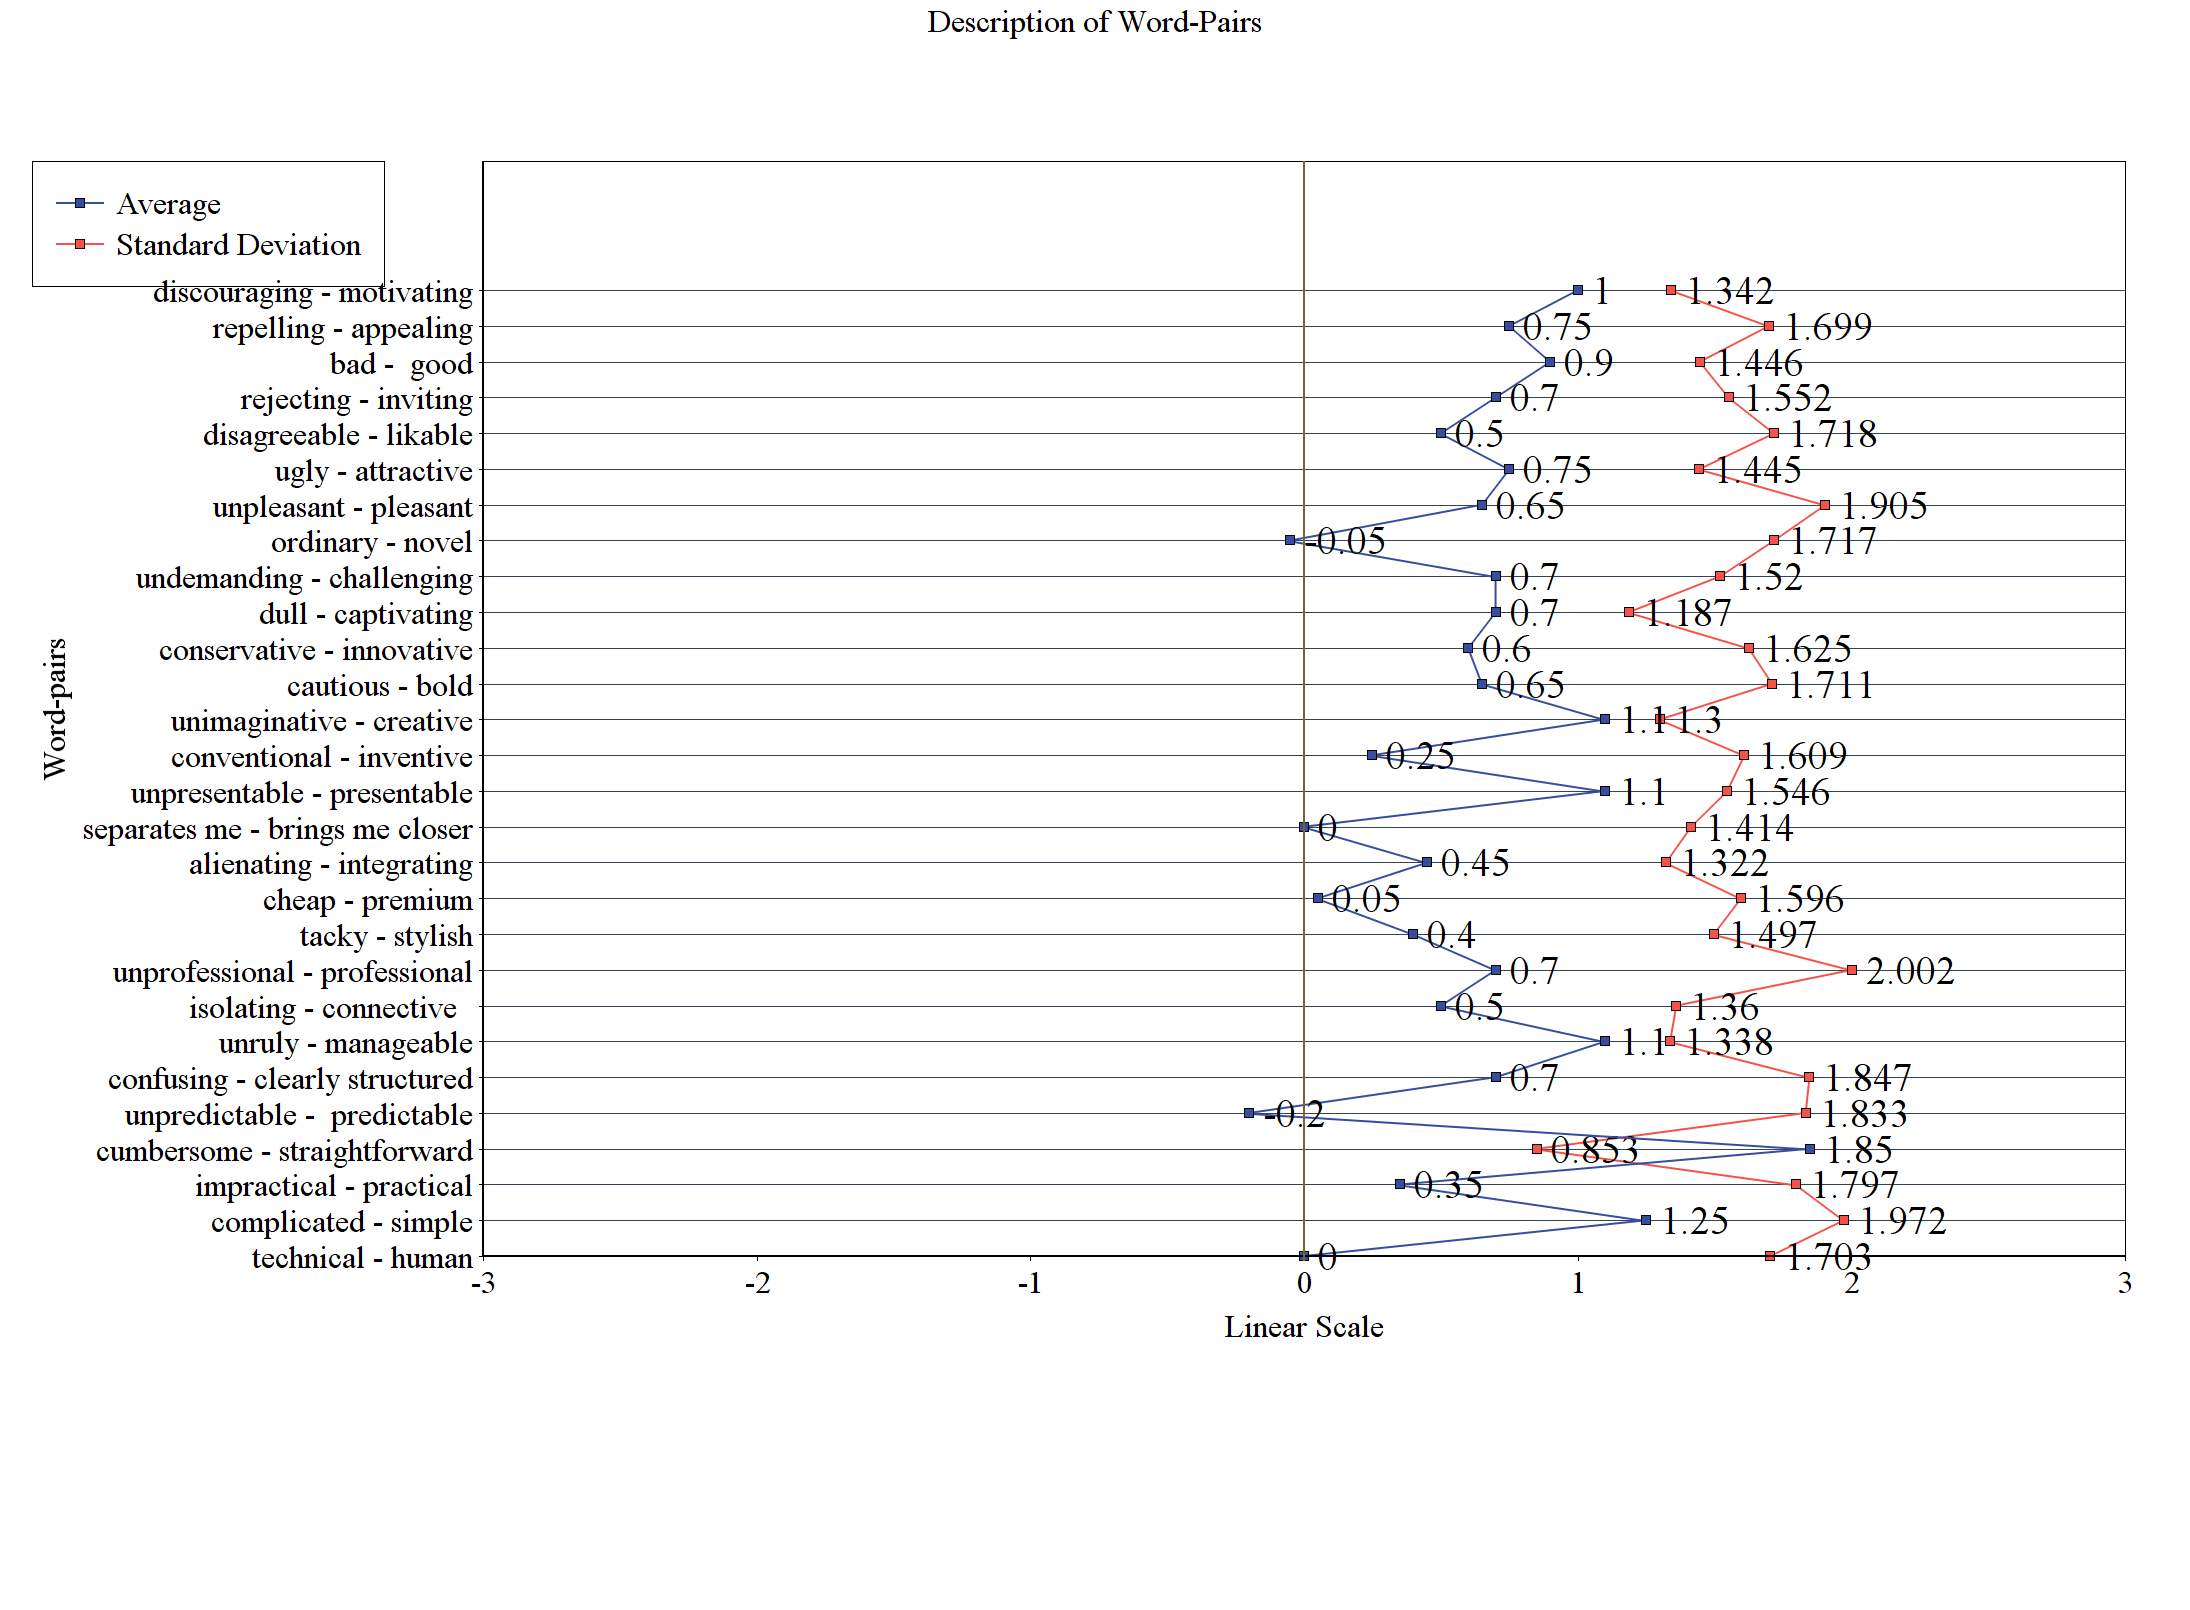
\includegraphics[width=1\textwidth]{img/Desc_of_Word_Pairs.png}
    \caption{Description of the word pairs along with the mean values and standard deviation \cite{attrakdiff}.}
    \label{fig:descofWordPair}
\end{figure}
\\~\\
The AttrakDiff questionnaire contains information for the pragmatic and hedonic quality of an interactive system. The language of the study was English but the participants also had an option for German.
\\~\\
As shown in Figure \ref{fig:descofWordPair}, the linear scale has been appointed the values from -3 to +3. The values -3 to -1 has been assigned to the negative aspect of the word pair e.g. "unpleasant". While 0 lies in the middle of the negative and positive aspects and referred to as neutral. Whereas, the range from +1 to +3 has been referred to the positive aspect of the word pair e.g. "pleasant".
\\~\\
The division of the word pairs according to their groups and classification with seven items each can also be inferred from Figure \ref{fig:descofWordPair}. The word pairs starting from "technical - human" till "unruly -manageable" lies under the pragmatic (PQ) category. Furthermore, word pairs from "isolating - connective" to "unpresentable - presentable" falls under the hedonic attribute group named Identification (HQ-I). Additionally, word pairs ranged from "conventional - inventive" and till "ordinary - novel" has been put under the shadow of hedonic stimulation (HQ-S). Lastly, Attractiveness (ATT) includes the set of the word pairs starting from "unpleasant - pleasant" and ending on "discouraging - motivating". 
\\~\\
Overall, the pragmatic quality for the chatbot rated by the participants is positive. It has been deduced from the results displayed in Figure \ref{fig:descofWordPair}. Respondents rated it neither technical nor human. The initial goal is achieved that at least the users didn't find it task-oriented or following some order. It is the first step towards more humanly. On the other hand, they are unable to discover their humanly characteristics. The possible reason for it could be a lack of ability to generate natural responses based on real communication. As it has been stuffed manually with a fixed number of responses. Moreover, the inadequate amount of data containing the limited number of intents (shown in Appendix \ref{appen:traindatastats}) has been used for training purposes. It could also be a reason for such feedback. Secondly, users rated it "Simple" with a positive mark greater than 1. The greatest peak at the positive side for the pragmatic section goes near to 2 for the term "Straightforward". Which means it was easy to understand and was uncomplicated. Moreover, users also found the chatbot practical, clearly structured, and manageable. The only negative point almost near to 0 has been encountered i.e. the chatbot is unpredictable. The possible reason for it could be the responses of the demo detective bot. But it has been designed like this for fun purposes. So by the results, it has been inferred that the users found the chatbot useful and assisting to achieve the desired goal.
\\~\\
Moving to the hedonic assessment, firstly hedonic identification ability (HQ-I) of the system has been tested using different word pairs that how the chatbot is delivering important personal values. It can also be inferred from the results portrayed in Figure \ref{fig:descofWordPair} that as a whole HQ-I appeared to be positive. The participants of this study graded the chatbot as connective, professional, stylish, integrating, and highly presentable. As the word pair "cheap - premium" is answered as neutral and it could be because of the shortness, unreality, and immaturity of dialogue due to the limitations of training data and responses. The positivity deduced from it is at least a chatbot is not ranked low in quality. Contrarily, neither it is rated as prime featured may be due to the definite dialogue topics or absence of any real-time achievement. Furthermore, ranking for "separates me - brings me closer" highlights that neither the majority felt isolated nor get apart with it nor they get attracted to it. It raised a need for improvement to make it more delivering and catchy for the users. It can be inferred from the overall analysis that the chatbot accomplished its task to deliver the values that users were expecting from it and fulfilled the users' expectations. But still there exist some areas that must be subjected to improvements.
\\~\\
Moreover, hedonic stimulation (HQ-S) has been used to measure the chatbot's challenging ability according to the users' perspective. Overall results for it have shown a positive trend. The users found it inventive, highly creative, bold, innovative, captivating, and challenging. But the arc for the term "ordinary - novel" has been graded as neutral. As users can see many other much improvised and state of the art chatbots like Google's Assistant, Apple's Siri, and Amazon's Alexa. So, they just considered it as a normal chatbot. It could be the reason that they neither rated it as ordinary nor novel. But instead of that by taking overall result into an account, the users found it challenging, interesting, and fascinating.
\\~\\
Finally, attractiveness has been measured for the chatbot by taking the results from PQ and HQ into consideration and by using separate related word pairs for it. By the results gathered from the participants' responses, it can be stated undoubtedly that all the users found it pleasant and attractive as the values for all the terms are positive. Which also makes it likable, inviting, good, appealing, and motivating.

\subsubsection*{Average Values}
According to Figure \ref{fig:avgValAttrak}, if the average values are considered to grade the quality of the chatbot then it is not wrong to say that attractiveness(ATT) has the highest value 0.75 and standard deviation(SD) of 0.15. While pragmatic quality(PQ) has been placed at second position with the mean value of 0.72 and SD of 0.67. On the other hand for hedonic quality's race, the challenging aspect of the chatbot is leading as hedonic stimulation(HQ-S) has the mean value 0.56 with SD as 0.34. Moreover, the chatbot succeeded in delivering the important values to the users at the lowest with an average of 0.46 and SD as 0.35. As it is not wrong to say that the initial chatbot has been rated well in all aspects. But the average values lie just under the category of lower positive. None of the sections collectively crossed the mark of +1 whereas the maximum limit that can be reached is +3. So, as the initial start, these results can be considered as good. But it will not be lame to say that the chatbot must go through some more training, structuring and designing to get improved in its next version to reach the desired level for its users.

\begin{figure}[!h]
    \centering
    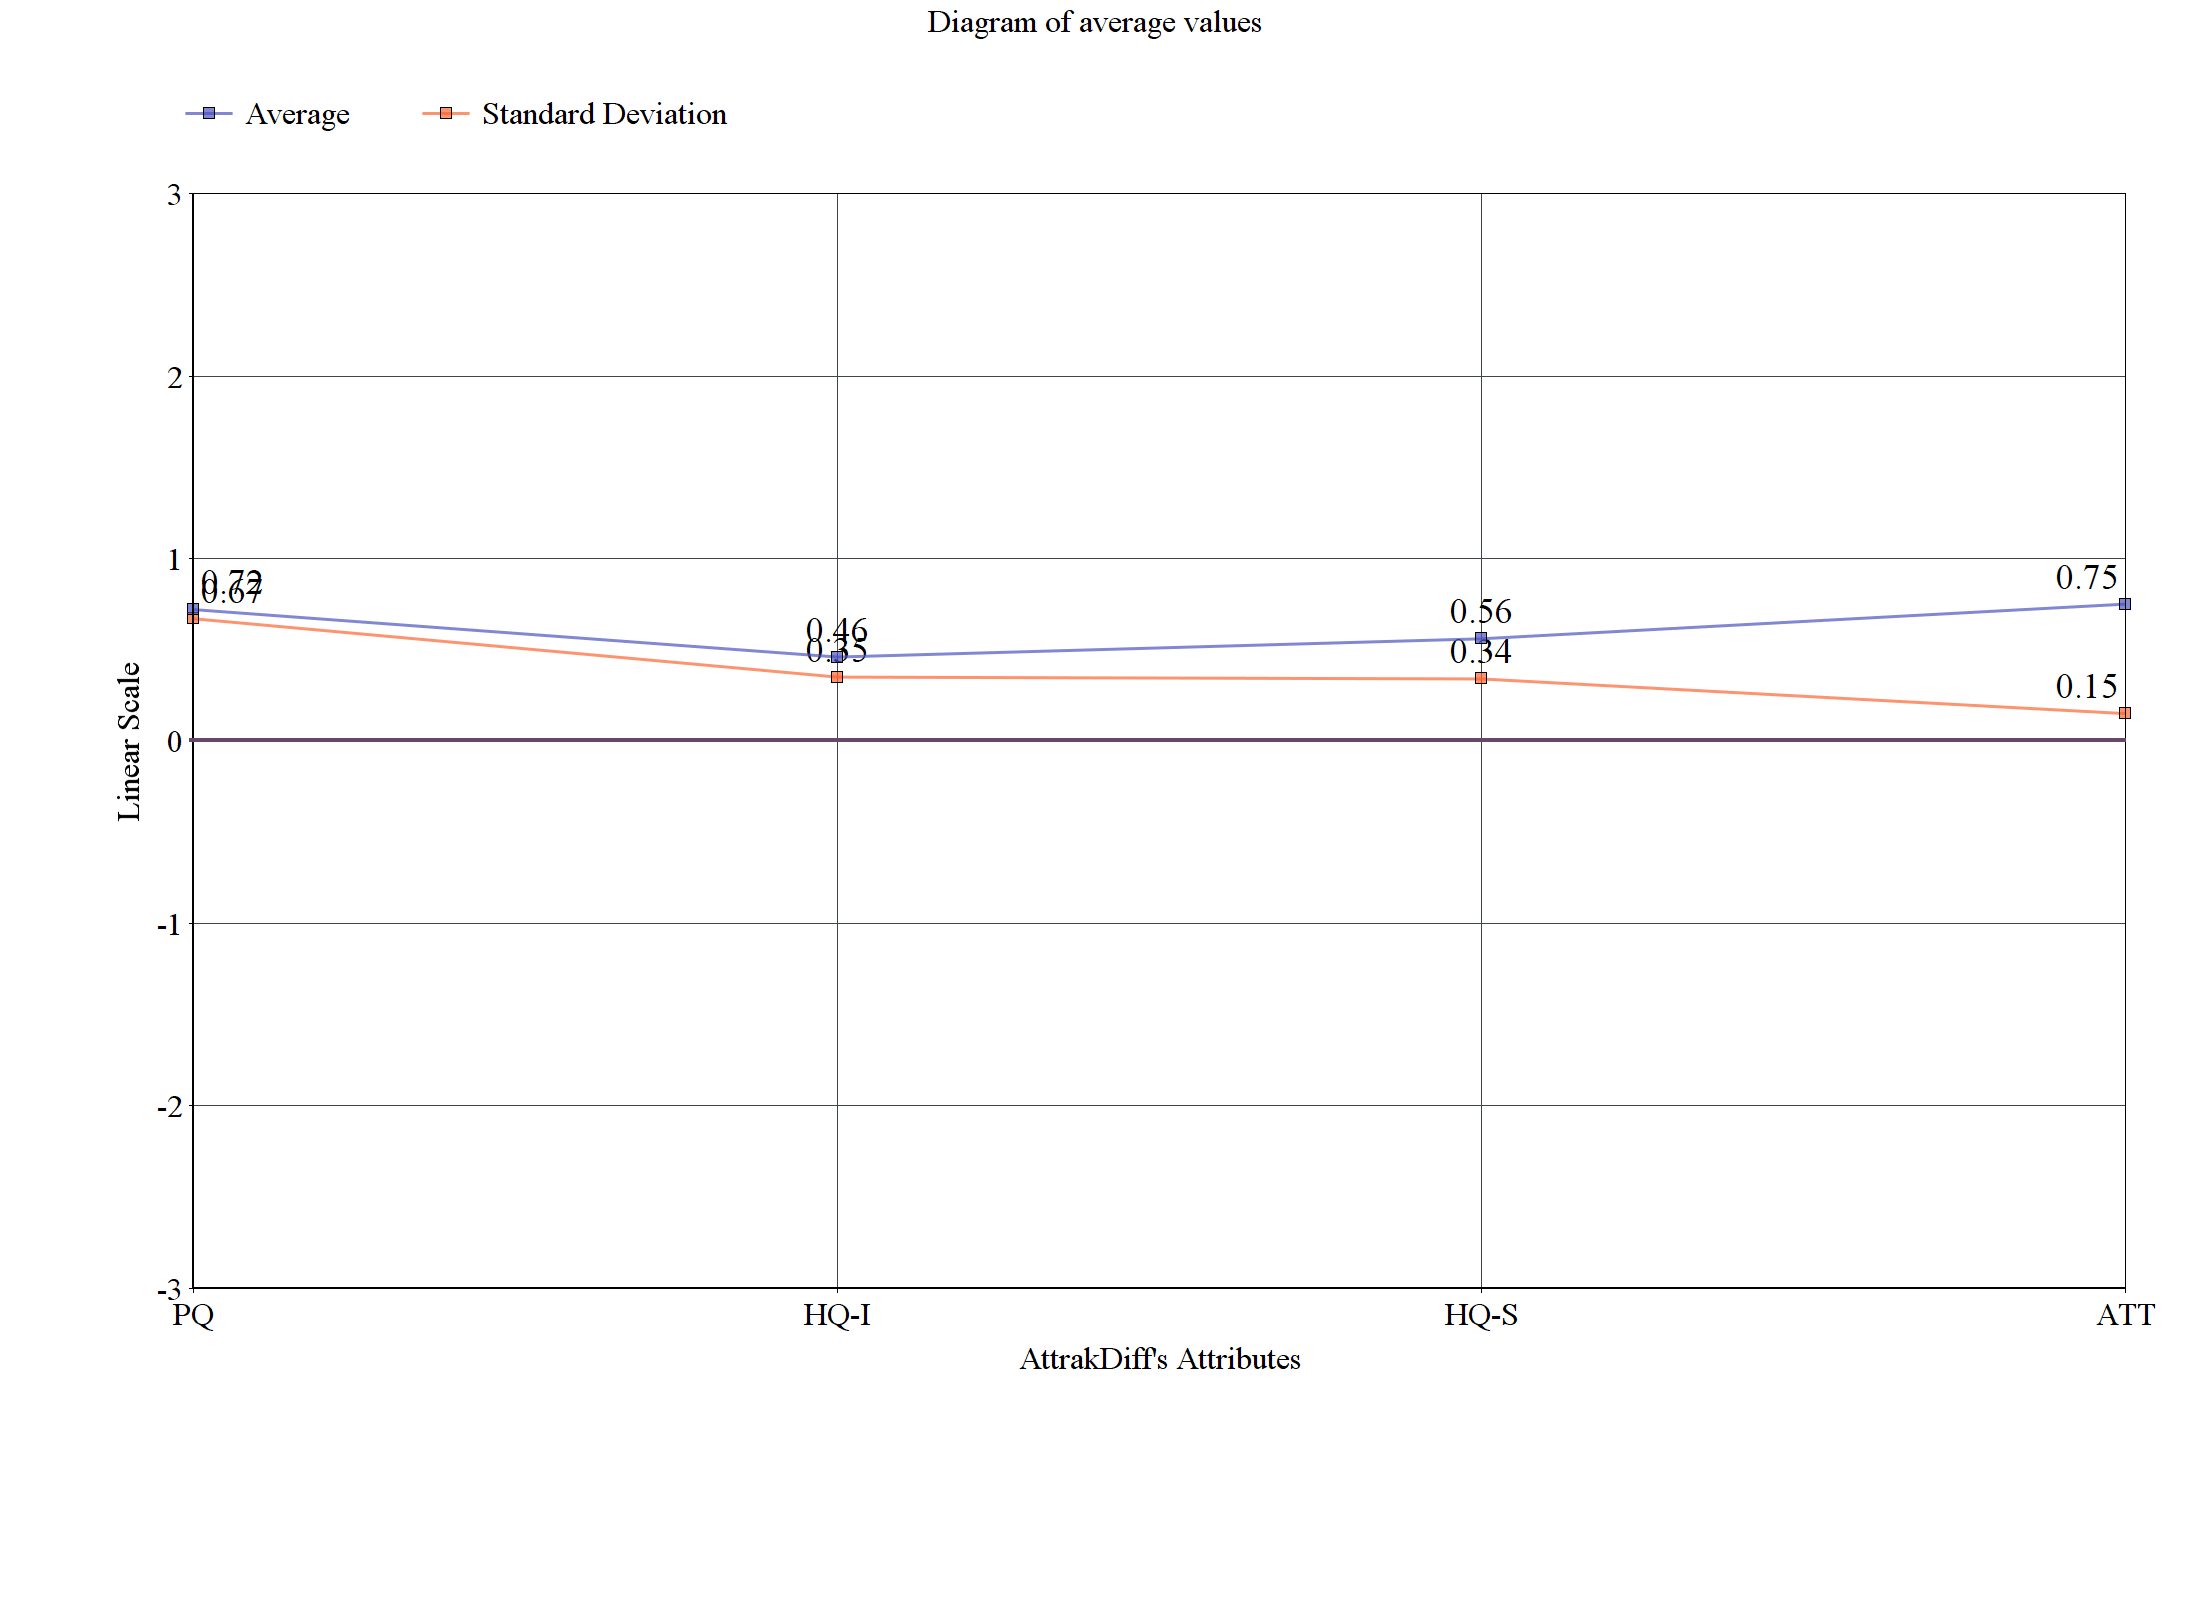
\includegraphics[width=0.8\textwidth]{img/Diagram_for_Avg_Values.png}
    \caption{Average values for PQ, HQ-I, HQ-S and ATT \cite{attrakdiff}.}
    \label{fig:avgValAttrak}
\end{figure}

\subsubsection*{Portfolio Discussion}
The dimensions for the portfolio of hedonic and pragmatic qualities have been displayed in Figure \ref{fig:portRes}. The vertical axis represents HQ(bottom = low value) while horizontal axis depicts PQ(left = low value). In the portfolio presentation, the outer bigger light blue rectangle is the confidence rectangle. It shows how divergent are the users in evaluating the product. The bigger is the confidence rectangle, the more diverged and less confident are the gathered results. The small dark blue spot is representing the actual rating of the system. The actual value for the PQ is 0.72 and HQ is 0.51. It can be visualized that the chatbot falls into the upper neutral area for both of the dimensions (PQ and HQ). Whereas, the confidence rectangle calculated by the users' agreement shows that the confidence interval for PQ is dispersed between neutral and task-oriented character-regions. Whereas, for HQ it falls below the self-oriented region. It illustrates that there is a room for optimization in both dimensions but more likely for HQ as compared to PQ. If the hedonic quality could be raised by optimizing the natural language understanding for the chatbot using enriched and sufficient training data. Then a user can communicate with it in a much better way and the chatbot can also be able to deliver its best and users could find it more joyful and delivering. Although, pragmatically it is touching the task-oriented area for now but still needs to be elevated by improving the provided assistance for the users to achieve their desired goals. By undergoing such enhancements it can reach the region of desired characteristics.

\begin{figure}[!h]
    \centering
    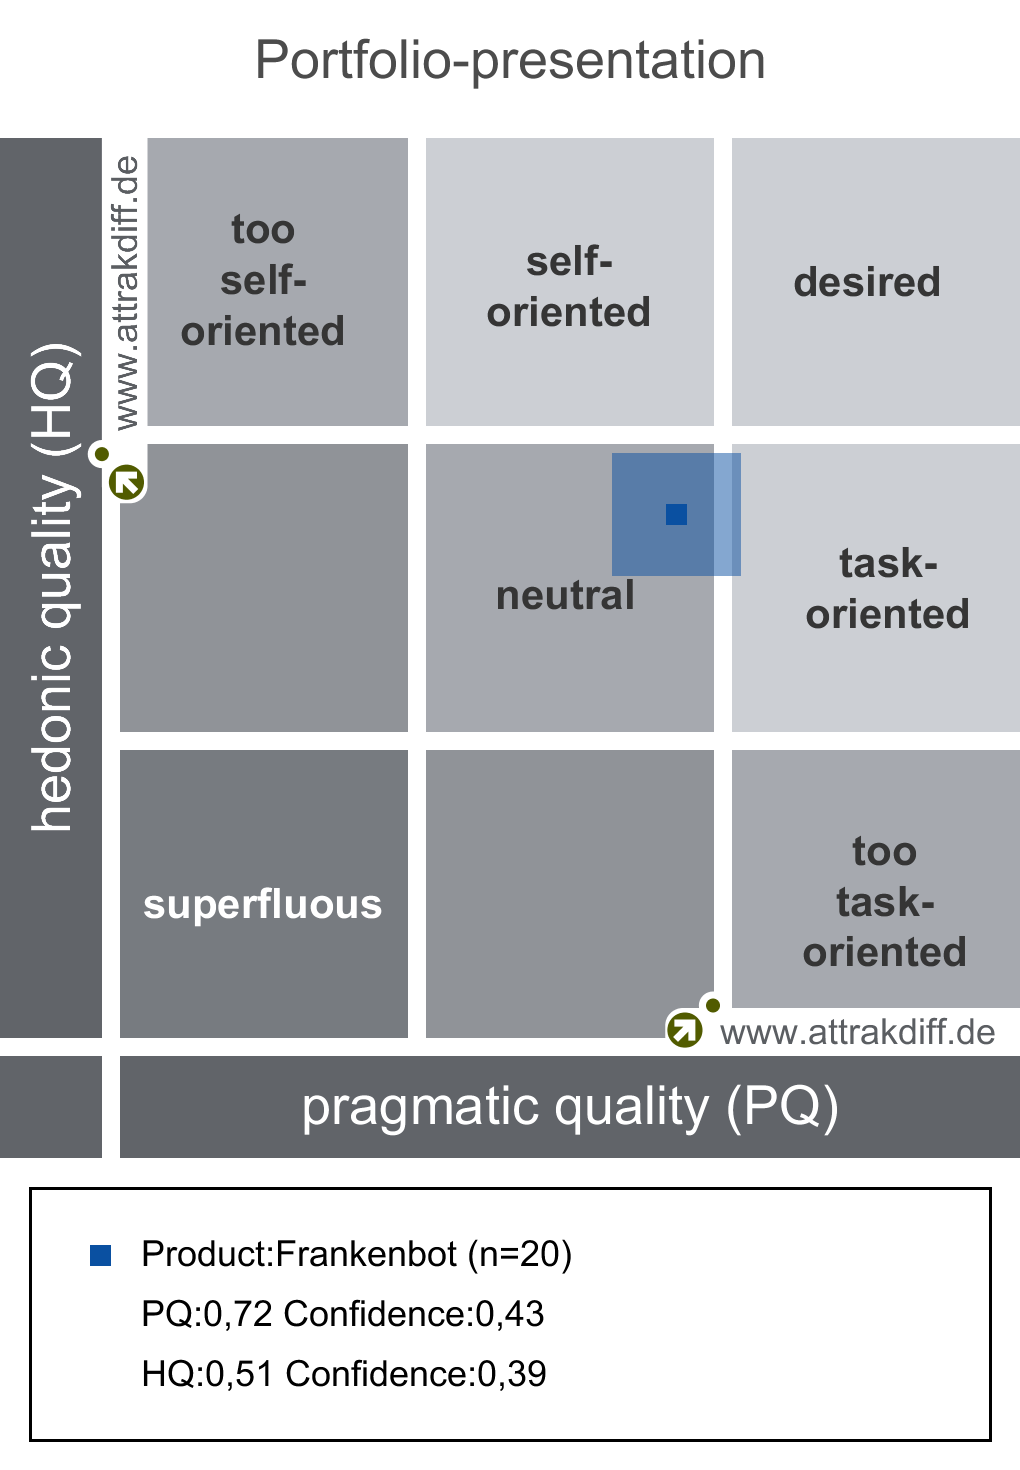
\includegraphics[width=0.7\textwidth]{img/Portfolio_of_results.png}
    \caption{Portfolio of the results for HQ and PQ of the chatbot \cite{attrakdiff}.}
    \label{fig:portRes}
\end{figure}

\section{Qualitative Analysis}
This section illustrates the incidents and behaviors that have been observed during the accomplishment of this research study. Some of the following characteristics have been noticed and reported in a verbal interview conducted by consulting 12 actors out of a total of 20 participants.

\subsection{Natural Language Understanding(NLU)}
It has been examined while performing self-testing on it that when the chatbot was inputted with the longer utterances, it was not able to identify the correct intent. Also whenever it has been asked for something that it is not trained for, the NLU was detecting the wrong intent. It is a real problem that could be a cause of confusion for the users and could also have made them lose their interest.
\\~\\
Out of total 12, 8 of the interviewed participants started the interaction with a greeting message and it worked well as the chatbot was designed so. But the remaining 4 tried to start the communication with any other statement and they reported that the chatbot was smart enough to guide them that how to start the conversation. All of them revealed that once the dialogue has been initiated they tried to enter longer utterances but overtime shortened their sentences due to irrelevant responses. And with shorter and simple utterances the chatbot produced relevant answers. The possible reason behind it is the NLU training using limited data.
\\~\\
10 out of a total of 12 interrogated users changed terms in a sentence to make the chatbot understand the correct semantics of their statements. But in the end, all of them were able to continue with the chat.

\subsection{Chatbot Guidance and Intelligence}
Also, 8 users reported that they were unable to move to the next question while playing a detective game but chatbot guided them well to make them understand what sort of input was it expecting from them at that specific moment. So, it can be deduced from it that the chatbot's ability to guide the user was good enough about the stuff for what it has not been trained or not expecting at some specific occasion. It was also able to deliver and to make the users understand its responses well. Furthermore, 7 of the users notified that they tried to deviate the chatbot from the topic but the detective didn't get diverted and forced them using convincing responses to put them back on track.

\subsection{Interaction}
A total of 12 participants were asked for feedback about their interaction with the chatbot. And 11 of them replied that it was fun and they enjoyed the communication with the chatbot. They also answered that the jokes it was cracking were joyful and made them laugh. Other than that they also liked the sarcasm and strictness in the responses of the detective bot as it was designed for making users feel that they are talking to some real detective. Only 1 out of 12 mentioned that the chatbot's answers were rude to some extent but when he was provided the reason for it then he realized and understood it. Conclusively, all the users who have been asked about the dialogue and the interaction with the chatbot loved it.

\subsection{Switching Topics}
As it was mentioned in the description of the chatbot to the users that the chatbot can talk about parallel topics at the same time. The users have to switch the topic and come back to the previous topic by answering the last question of that topic at any moment in the future. When the users have been asked about it in verbal conversation, all(12) of them mentioned that it worked fine and they liked and appreciated this feature.

\subsection{Detective Game}
The same 12 participants have also been questioned to gather feedback about detective games whether they liked it or not. To be precise, 6 out of them liked it and the other 4 complaints about the short length of the game and the scenario were not directed well. In addition to it, the remaining 2 found it as a source of recreation for them. Cumulatively, all of them liked the idea of the detective game as a demo. Also, the users have been requested to end the game before moving to the completion of the surveys. And all of them replied positively on asking whether they reached an end of the game before filling out the questionnaires.

\subsection{User Interface}
9 out of the total 12 participants liked the interface. But the remaining 3 of them disliked it due to the dark theme as they recommended the light-colored scheme for it. Otherwise, all of the users liked the design and style of an interface.  


